\documentclass[10pt,spanish]{article}

%----------------------------------------------------------------------------------------
% Codificación, y usar una fuente similar a la Palatino (y no Latin Modern Roman)
\usepackage[utf8]{inputenc} % Acentos, etc.
\usepackage[spanish]{babel} % Castellano
\usepackage[T1]{fontenc}
\renewcommand{\rmdefault}{phv} % Arial (se parece lo suficiente)
\renewcommand{\sfdefault}{phv} % Arial (se parece lo suficiente)

%----------------------------------------------------------------------------------------
% Margenes
\usepackage{geometry}
\geometry{
    a4paper,
    total={210mm,297mm},
    left=30mm,
    right=30mm,
    top=25mm,
    bottom=25mm,
}

%----------------------------------------------------------------------------------------
% Modificar tanto el estilo de las secciones como del indice
\usepackage{titlesec}
\titleformat{\section}{\bfseries\Large\uppercase}{\thesection .}{0.8em}{}
\titleformat{\subsection}{\bfseries\large}{\thesubsection .}{0.8em}{}
\titleformat{\subsubsection}{\bfseries}{\thesubsubsection .}{0.8em}{}
%\newcommand{\sectionbreak}{\clearpage} % Empezar secciones en nueva página

%----------------------------------------------------------------------------------------
% Indentar primera línea párrafos
\usepackage{indentfirst}

%----------------------------------------------------------------------------------------
% Colores
\usepackage{xcolor,colortbl} % Colores personalizados y color fondo tablas
\definecolor{grisCabeceraTabla}{RGB}{220,220,220}
\definecolor{grisHeader}{RGB}{180,180,180}

%----------------------------------------------------------------------------------------
% Imagenes: Que se pongan donde yo quiero
\usepackage{graphicx}
%\usepackage{float}
\usepackage[linecolor=colComment,linewidth=0.65pt]{mdframed}

\usepackage{floatpag} % Pagina en blanco cuando aparece figuras.

\DeclareGraphicsExtensions{.svg,.eps,.ps,.pdf,.png,.jpg,.jpeg}
\addto{\captionsspanish}{\renewcommand{\listfigurename}{\bfseries\Large Figuras}}


%----------------------------------------------------------------------------------------
% FANCY HEADER
\usepackage{fancyhdr}
\pagestyle{fancy}
\fancyhf{} % borrar todos los ajustes

% Configurar la cabecera: fancyhead, fancyfoot para el pie.
\fancyhead[R]{\nouppercase 30243-Proyecto Software 13/14 – Equipo {\bf 20}}
\renewcommand{\headrulewidth}{0pt} % Tam. separador cabecera
\renewcommand{\footrulewidth}{0pt}   % Tam. separador pie
\renewcommand{\headwidth}{6in}       % Anchura cabecera (incluido separador)

%----------------------------------------------------------------------------------------
% Curriculum Vitae
\usepackage{currvita} 
\setlength{\cvlabelwidth}{40mm}

%----------------------------------------------------------------------------------------
% Tablas (entre otras, las actas de las reuniones)
\linespread {1.4} % Tamaño que ocupa una línea (celda)

\usepackage{array}
\usepackage{longtable}
\setlength\LTleft{0pt}
\setlength\LTright{0pt}
\setlength{\columnsep}{0em}

% Definir los estilos de las celdas para indentar el texto
\newcolumntype{L}[1]{>{\raggedright\let\newline\\\arraybackslash\hspace{0pt}}m{#1}}
\newcolumntype{C}[1]{>{\centering\let\newline\\\arraybackslash\hspace{0pt}}m{#1}}
\newcolumntype{R}[1]{>{\raggedleft\let\newline\\\arraybackslash\hspace{0pt}}m{#1}}

% Filas con columnas multiples
\newcommand{\mc}[2]{\multicolumn{#1}{|C{\dimexpr 1\linewidth-2\tabcolsep}|}{#2}}

% Colores de lineas de las tablas
\arrayrulecolor{grisHeader}

% Eliminar espacio previo en lista de ítems
\usepackage{enumitem}
\setlist{nolistsep}

% Comandos especiales para crear items dentro de tabla y poder hacer
% una tabla de multiples paginas y que se pueda realizar el salto de
% pagina en cualquier punto.
\usepackage{scrextend}
\newcommand{\cabeceraTabla}[1]{\rowcolor{grisCabeceraTabla}{\bf #1}}
\newcommand{\espacioSubtabla}{\\[0.5ex]}

\newenvironment{lvlOneItem}
	{\begin{addmargin}[2.5em]{1em}
	\vspace{-1em}
	\hspace{-1em}$\bullet$\hspace{0.5em}}
	{\vspace{-2em}\end{addmargin}}
\newenvironment{lvlTwoItem}
	{\begin{addmargin}[4em]{1em}
	\vspace{-1em}
	\hspace{-1em}$\circ$\hspace{0.5em}}
	{\vspace{-2em}\end{addmargin}}
\newenvironment{lvlThreeItem}
	{\begin{addmargin}[5.5em]{1em}
	\vspace{-1em}
	\hspace{-1em}$\blacktriangleright$\hspace{0.5em}}
	{\vspace{-2em}\end{addmargin}}

\newcommand{\itemNvlUno}[1]{\begin{lvlOneItem}{#1}\end{lvlOneItem}\\}
\newcommand{\itemNvlDos}[1]{\begin{lvlTwoItem}{#1}\end{lvlTwoItem}\\}
\newcommand{\itemNvlTres}[1]{\begin{lvlThreeItem}{#1}\end{lvlThreeItem}\\}

%----------------------------------------------------------------------------------------
% Definir el titulo
\newcommand{\nombreDelProyecto}{$\mu Search$}


\newcommand{\singlelinebreak}{\\[\baselineskip]}
\newcommand{\multiplelinebreak}[1]{\\[#1\baselineskip]}
\newlength{\drop}

\newcommand*{\titulo}{\begingroup
\thispagestyle{empty}
\drop = 0.13\textheight
\centering
\vfill
\vspace*{\drop}

\includegraphics[scale=0.25]{img/bitparty_big}\singlelinebreak
{\Huge\bf BITPARTY}\multiplelinebreak{2}
{\huge Proyecto \nombreDelProyecto}\multiplelinebreak{2}
{\Large Versión  1.0}\multiplelinebreak{1}
{\Large 06/2014}\multiplelinebreak{1}
{\em Alberto Berbel Aznar}\\
{\em Javier Briz Alastrué}\\
{\em Héctor Francia Molinero}\\
{\em Daniel García Páez}\\
{\em Alejandro Gracia Mateo}\\
{\em Simón Ortego Parra}\multiplelinebreak{6}

\includegraphics[scale=0.09]{img/diis_uz_big}\singlelinebreak
\vfill
\vspace*{\drop}
\endgroup}

%----------------------------------------------------------------------------------------
% Metadatos y pdf clickeable
\usepackage{hyperref}
\usepackage{hyperxmp}

\newcommand{\numeroDeReunion}{01}
\newcommand{\tituloReunion}{\bf Lanzamiento del equipo}

\hypersetup{
	pdfauthor={Alberto Berbel Aznar, 
				Javier Briz Alastrué, 
				Héctor Francia Molinero, 
				Daniel García Páez,
				Alejandro Gracia Mateo,
				Simón Ortego Parra},
	pdftitle={E20 - Propuesta del proyecto},
	pdfsubject={Proyecto Software. Grado Ing. Informática. EINA. Unizar},
	pdfkeywords={},
	pdfcopyright={Copyright \copyright\ 2014 
				Alberto Berbel Aznar, 
				Javier Briz Alastrué, 
				Héctor Francia Molinero, 
				Daniel García Páez,
				Alejandro Gracia Mateo,
				Simón Ortego Parra. All rights reserved.},
	pdfproducer={PDFLatex},
	pdfcreator={ps2pdf},
	colorlinks=true
}

% Redefinir el nombre de referencias a lo largo del documento
\usepackage[capitalise]{cleveref} % IMPORTANT: load after hyperref package
\crefdefaultlabelformat{\textbf{#2#1#3}} % boldface only the number

\crefname{figure}{figura}{figuras}
\Crefname{figure}{Figura}{Figuras}
\crefname{listing}{algoritmo}{algoritmos}
\Crefname{listing}{Algoritmo}{Algoritmos}
\crefname{section}{sección}{secciones}
\Crefname{section}{Sección}{Secciones}

% Varios comandos a links relativos a otros ficheros (xls, pdf's, etc.)
\newcommand{\hojaesfuerzos}[2]{\href{run:xls/#1.xls}{#2}}%

%=-=-=-=-=-=-=-=-=-=-=-=-=-=-=-=-=-=-=-=-=-=-=-=-=-=-=-=-=-=-=-=-=-=-=-=-=-=-=-=-=-=-=-=-=-=-=%
%           I  N  I  C  I  O           D  E  L           D  O  C  U  M  E  N  T  O            %
%=-=-=-=-=-=-=-=-=-=-=-=-=-=-=-=-=-=-=-=-=-=-=-=-=-=-=-=-=-=-=-=-=-=-=-=-=-=-=-=-=-=-=-=-=-=-=%

% Comenzar sin numeracion en las paginas
\renewcommand{\thepage}{}

\usepackage{blindtext} % TEXTO DE RELLENO PARA PLANTILLA

%==============================================================================================
% PORTADA
%==============================================================================================

\begin{document}
\titulo
\clearpage

%==============================================================================================
% ÍNDICE
%==============================================================================================	

\newpage
\thispagestyle{empty}
\mbox{}
\tableofcontents

% Continuar con numeracion romana (1,2,3...) 
\renewcommand{\thepage}{\arabic{page}}

%==============================================================================================
% 01.   INTRODUCCIÓN
% 01.1. IDENTIFICACIÓN DEL PROYECTO
% 01.2. OBJETIVO Y ALCANCE DEL PROYECTO
% 01.3. IDENTIFICACIÓN DEL EQUIPO QUE REALIZA EL PROYECTO
% 01.4. BREVE DESCRIPCION DEL CONTENIDO DEL RESTO DE SECCIONES DE LA MEMORIA, INCLUYENDO ANEXOS
%==============================================================================================

% 01
\fancyfoot[C]{\thepage}
\section{Introducción}
% 01. INTRODUCCIÓN
%==============================================================================================

\blindtext
% 01.1
\subsection{Identificación del proyecto}
% 01.1. IDENTIFICACION DEL PROYECTO
%----------------------------------------------------------------------------------------------

\blindtext
% 01.1
\subsection{Objetivo y alcanze}
% 01.2. OBJETIVO Y ALCANCE DEL PROYECTO
%----------------------------------------------------------------------------------------------
La presente aplicación tiene como objetivo dar solución al problema planteado por la empresa cliente.
El cliente nos ha transmitido la necesidad de diseñar un catálogo electrónico de los microconroladores que distribuye, que permita la gestión de los productos disponibles, y que permita a los clientes realizar búsquedas y efectuar pedidos.
\blindtext
% 01.1
\subsection{Identificación del equipo}
% 01.3. IDENTIFICACIÓN DEL EQUIPO QUE REALIZA EL PROYECTO
%----------------------------------------------------------------------------------------------

\blindtext
% 01.4
\subsection{Descripción del contenido}
% 01.4. BREVE DESCRIPCION DEL CONTENIDO DEL RESTO DE SECCIONES DE LA MEMORIA, INCLUYENDO ANEXOS
%----------------------------------------------------------------------------------------------
En la presente memoria se detallan todos los aspectos referentes a la aplicación y al proceso de su desarrollo.

Se detallan los requisitos que el cliente plateó inicialmente para el sistema, la descripción técnica de la solución adoptada, lsa pruebas que se han realizado para verificar que los requisitos se cumplen, los manuales generados, tanto el manual técnico como el de usuario.

También se detallan en esta memoria todas las actividades llevadas a cabo en el proyecto, incluidas las reuniones y sus actas y otra documentación generada en ellas, así como las configuraciones que se han utilizado en el proyecto.

Finalmente se explican las prácticas llevadas a cabo con el fin de asegurar la calidad de la aplicación y se concluye este documento comentando las lecciones aprendidas en el transcurso del proyecto y las conclusiones extraidas del mismo.

Se anexan los curriculum vitae de los miembros del equipo, las hojas de esfuerzo de cada uno de ellos, y otros documentos que aportan información adicional a secciones anteriormente mencionadas.
\blindtext
%==============================================================================================
% 02. REQUISITOS DEL SISTEMA
%==============================================================================================

% 02
\section{Requisitos del sistema}
% 02. REQUISITOS DEL SISTEMA
%==============================================================================================

\blindtext
%==============================================================================================
% 03.   DESCRIPCIÓN TÉCNICA
% 03.1. ASPECTOS ARQUITECTURALES Y TECNOLOGICOS
% 03.2. MODELOS DE DATOS
% 03.3. INFORMACIÓN DE DISEÑO DE COMPONENTES RELEVANTES DEL SISTEMA
%==============================================================================================

% 03
\section{Descripción técnica}
% 03. DESCRIPCIÓN TÉCNICA
%==============================================================================================
La solución técnica que se ha dado con el desarrollo de este proyecto está basada en tecnologías web, capaces de resolver tanto los requisitos de interacción de la aplicación con el usuario como los problemas relacionados con tratamiento y persistencia interna de la información.
Concretamente, se utilizará una interfaz web compatible con las últimas versiones de los navegadores más utilizados (más adelante se detallará esto), y se utilizará el framework CodeIgniter, en lenguaje PHP, como base del proyecto. Para el almacenamiento de la información se utilizará una base de datos MySQL.
Para evitar problemas de latencias con la base de datos, y dado el reducido tamaño del sistema, se optará por alojar la base de datos y todo el resto del sistema (servidor web e intérprete PHP) en un mismo servidor.

Las tecnologías, lenguajes y aplicaciones utilizadas en el desarrollo del proyecto han sido:

\begin{itemize}
\item HTML 5
\item CSS 3
\item PHP 5
\item CodeIgniter 2.1.4
\item MySQL 5.5
\end{itemize}

Se ha asegurado que la web renderice de forma correcta en los siguientes navegadores:

\begin{itemize}
\item Google Chrome >=30
\item Internet Explorer >=10
\item Mozilla Firefox >=27
\item Opera >=12
\end{itemize}

La documentación y manuales de usuario se entregaran al cliente en formato PDF.


\blindtext
% 03.1
\subsection{Aspectos arquitecturales y tecnológicos}
% 03.1. ASPECTOS ARQUITECTURALES Y TECNOLOGICOS
%----------------------------------------------------------------------------------------------

\blindtext
% 03.2
\subsection{Modelos de datos}
% 03.2. MODELOS DE DATOS
%----------------------------------------------------------------------------------------------
\paragraph{}Nuestro modelo de datos es muy sencillo puesto que solo necesitamos almacenar en la base de datos la información relacionada con los microcontroladores. El resto de la información que manejamos no se almacena en nuestra base de datos; los microcontroladores que introduce un usuario en el carrito de  la compra, los guardamos temporalmente utilizando las funciones de PHP; y la información asociada a un  cliente que realiza una compra, no se almacena en ningún sitio puesto que solo queda reflejada en la factura que se genera cuando se solicita un pedido. \newline

\noindent Por lo tanto, nuestro modelo de datos es el siguiente:

\begin{figure}[h!]
\centering
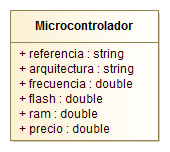
\includegraphics[width=0.40\textwidth]{img/modelo_datos}
\caption{Modelo de datos}
 \label{fig:modelo_datos}
\end{figure}

\blindtext
% 03.3
\subsection{Diseño de los componentes}
% 03.3. INFORMACIÓN DE DISEÑO DE COMPONENTES RELEVANTES DEL SISTEMA
%----------------------------------------------------------------------------------------------
Los componentes relevantes del sistema son los que ya han sido explicados en el apartado de Aspectos Arquitecturales y Tecnológicos, propios del patrón de diseño de Modelo-Vista-Presentador. Hemos elegido este patrón de diseño porque consideramos que es un patrón que se ajusta perfectamente al problema que tenemos que resolver y a su vez ofrece una solución lo más sencilla posible.

\vspace{.2cm}
\begin{figure}[ht]
\centerline{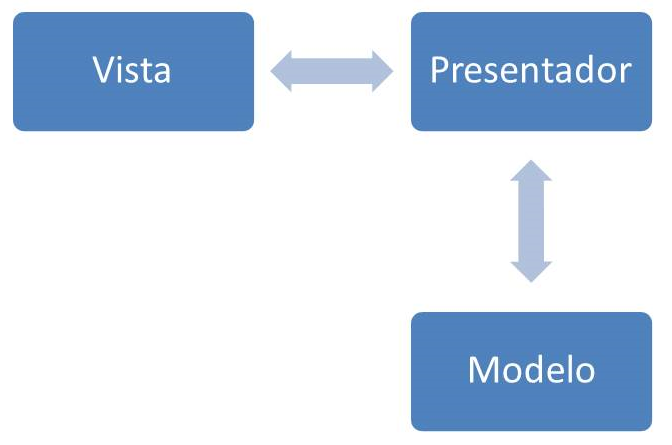
\includegraphics[scale=0.6]{img/componentes}}\
\caption{Componentes relevantes del sistema}
\label{fig:diagCompon}
\end{figure}
\blindtext
%==============================================================================================
% 04.   VERIFICACIÓN Y VALIDACIÓN DEL SISTEMA
% 04.1. DESCRIPCIÓN DE LA METODOLOGÍA SEGUIDA PARA LA REALIZACIÓN DE LAS PRUEBAS DEL SISTEMA
% 04.2. PRUEBAS REALIZADAS, DEFECTOS ENCONTRADOS Y CAMBIOS Y CORRECCIONES QUE HA HABIDO
%       QUE REALIZAR. EN ESTA SECCIÓN O EN ANEXO LOS INFORMES DE TODAS LAS PRUEBAS.
%==============================================================================================

% 04
\section{Verificación y validación}
% 04. VERIFICACIÓN Y VALIDACIÓN DEL SISTEMA
%==============================================================================================
\blindtext
% 04.1
\subsection{Metodología de pruebas}
% 04.1. DESCRIPCIÓN DE LA METODOLOGÍA SEGUIDA PARA LA REALIZACIÓN DE LAS PRUEBAS DEL SISTEMA
%----------------------------------------------------------------------------------------------
Puesto que para la realización de las pruebas hemos utilizado nuestros conocimientos previos adquiridos en la aplicación de Validación y Verificación en otros proyectos, para no desviarnos de lo conocido, nuestra metodología de pruebas se aproxima a la metodología de pruebas utilizada en dichos proyectos anteriores: TMAP Next (Test Management Approach).
\\[6pt]
Los fundamentos de TMAP se basan en cuatro elementos esenciales:
\begin{itemize}
	\item \textbf{Proceso dirigido por el negocio.} La economía marca el esfuerzo a realizar, y cuáles son los riesgos prioritarios.
	\item \textbf{Un proceso de pruebas estructurado.} Nos guía a la hora de responder a las cuestiones típicas de \textit{qué/cuándo, cómo, con qué y quién} (ciclo de vida de pruebas).
	\item \textbf{Un kit de herramientas.} Se ofrece información práctica para establecer la infraestructura (\textit{con qué}), las técnicas (\textit{cómo}), y la organización (\textit{quién}).
	\item \textbf{Método completo y adaptable.} Flexibilidad para adaptar la metodología a distintas situaciones de desarrollo: nuevos desarrollos, mantenimiento, desarrollo propio o basado en software comercial, ...
\end{itemize}
\paragraph{} Pasos a dar en la gestión de pruebas dirigida por el negocio:
\begin{enumerate} 
	\item Identificar los objetivos de las pruebas
	\item Determinar los riesgos
	\item Determinar si una característica/parte se debe probar de forma detallada o ligera
	\item Estimar y planificar
	\item Elegir las técnicas de prueba y ejecutarlas 
	\item Informar sobre el progreso, calidad
\end{enumerate}

\blindtext
% 04.2
\subsection{Pruebas. Defectos. Correcciones}
% 04.2. PRUEBAS REALIZADAS, DEFECTOS ENCONTRADOS Y CAMBIOS Y CORRECCIONES QUE HA HABIDO
%       QUE REALIZAR. EN ESTA SECCIÓN O EN ANEXO LOS INFORMES DE TODAS LAS PRUEBAS.
%----------------------------------------------------------------------------------------------

\blindtext
%==============================================================================================
% 05.   MANUALES
% 05.1. MANUAL DE USUARIO
% 05.1. MANUAL DE INSTALACIÓN
%==============================================================================================

% 05
\section{Manuales}
% 05. MANUALES
%==============================================================================================

\paragraph{}En este apartado se presentan los manuales de usuario necesarios para que tanto el usuario cliente de la aplicación como el administrador de la misma aprendan a utilizarla y navegar por ella de la forma más rápida y sencilla posible.

\paragraph{}Además se añade un manual de instalación para que, en caso de que la empresa cliente a la que va dirigida este producto decida mantener ella el catálogo electrónico, pueda instalar y preparar el entorno necesario para ello.
\blindtext
% 05.1
\subsection{Manual de usuario}
% 05.1. MANUAL DE USUARIO
%----------------------------------------------------------------------------------------------
El manual de usuario, incluye dos versiones conjuntas en un mismo documento:
\begin{itemize}
	\item La del usuario cliente que utilzará la aplicación para navegar por la misma y realizar sus compras de microcontroladores
	\item La del usuario administrador de la empresa cliente que tendrá acceso interno al catálogo electronico para añadir, modificar y eliminar microcontroladores del mismo.
\end{itemize}

Se puede acceder a él a través del \manualUsuario{guia_usuario}{siguiente enlace}.

\blindtext
% 05.2
\subsection{Manual de instalación}
% 05.2. MANUAL DE INSTALACIÓN
%----------------------------------------------------------------------------------------------
Al manual de instalación se puede acceder a través del siguiente enlace.
\blindtext
%==============================================================================================
% 06.     GESTIÓN DEL PROYECTO
% 06.1.   FASES Y ACTIVIDADES DEL PROYECTO
% 06.1.1. RIESGOS
% 06.1.2. ESTIMACIONES GLOBALES DE TAMAÑOS Y ESFUERZOS INICIALES
% 06.1.3. CRONOGRAMAS GLOBAL INICIAL Y FINAL
% 06.1.4. TAREAS Y ESTIMACIONES DE ESFUERZOS POR ITERACIÓN 
% 06.1.5. FICHEROS DE ESFUERZOS INDIVIDUALES 
% 06.1.6. ESFUERZOS REALES DE LAS TAREAS POR ITERACIÓN 
% 06.1.7. ESFUERZOS REALES DE LAS PERSONAS Y ROLES 
% 06.2.   PROCESOS DE SEGUIMIENTO Y CONTROL
% 06.2.1. CALENDARIO DE LAS DISTINTAS REUNIONES CELEBRADAS
% 06.2.2. ACTAS DE LAS DISTINTAS REUNIONES CELEBRADAS
% 06.3.   COSTE REAL DEL PROYECTO
%==============================================================================================

% 06
\section{Gestión del proyecto}
% 06. GESTIÓN DEL PROYECTO
%----------------------------------------------------------------------------------------

\blindtext
% 06.1
\subsection{Fases y actividades}
% 06.1. FASES Y ACTIVIDADES DEL PROYECTO
%----------------------------------------------------------------------------------------
En esta sección se explican las diferentes partes por las que ha pasado el proyecto, cómo se han planificado, qué tareas se han realizado en cada fase y que esfuerzos han supuesto llevarlas a cabo.
\blindtext
% 06.1.1
\subsubsection{Riesgos}
% 06.1.1. RIESGOS
%----------------------------------------------------------------------------------------

\blindtext
% 06.1.2
\subsubsection{Estimaciones iniciales}
% 06.1.2. ESTIMACIONES GLOBALES DE TAMAÑOS Y ESFUERZOS INICIALES
%----------------------------------------------------------------------------------------

\paragraph{} Se muestra en la figura \ref{fig:6121} los tiempos que se han asignado a las diferentes tareas. En esta figura se muestran las horas concretas que se estimaron al principio del proyecto. Más adelante se mostrara cuantas horas reales se invirtieron en cada apartado.

\begin{figure}[h!]
\centering
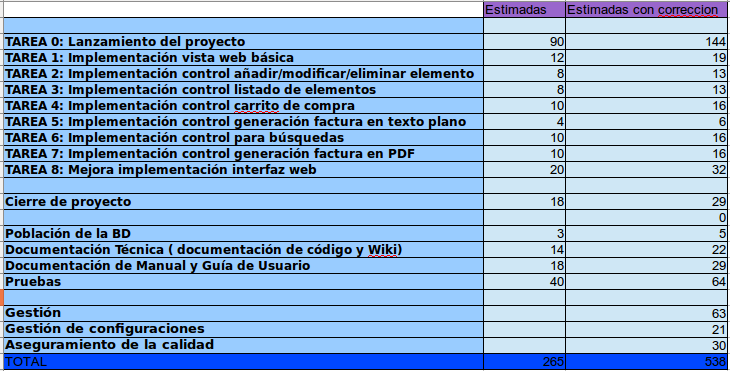
\includegraphics[width=0.95\textwidth]{img/6121}
\caption{Estimación esfuerzos totales}
 \label{fig:6121}
\end{figure}

\paragraph{} Se muestra en la figura \ref{fig:6122} las horas asignadas a cada una de las tareas. Se puede ver que las partes más costosas son sobre todo el lanzamiento del proyecto,gestión y pruebas.Implementación se llevaría otra de las grandes partes del proyecto, pero al estar dividida en subtareas parece que ocupe un tiempo menor del que en realidad lleva.

\begin{figure}[h!]
\centering
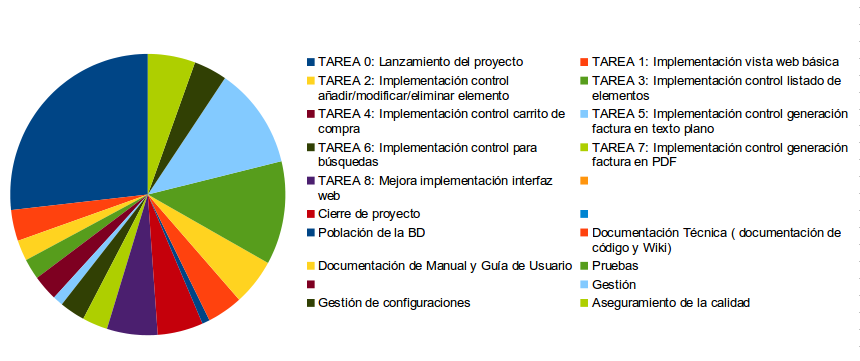
\includegraphics[width=0.95\textwidth]{img/6122}
\caption{Gráfica esfuerzos totales}
 \label{fig:6122}
\end{figure}
\blindtext
% 06.1.3
\subsubsection{Cronogramas}
% 06.1.3. CRONOGRAMAS GLOBAL INICIAL Y FINAL
%----------------------------------------------------------------------------------------

\paragraph{} Se pueden visualizar, tanto el cronograma que se planificó inicialmente y como el cronograma que resulto finalmente, en el anexo \ref{sec:cronogramas} de este documento. 
\paragraph{}En general las tareas se retrasaron un poco frente a la planificación prevista, tanto su comienzo como su finalización. Pero siempre se ha ido desarrollando el proyecto con los tiempos previstos y cumpliendo los objetivos adecuadamente. Alguna de las tareas se pudo alargar algo más en el tiempo que lo mostrado en el cronograma, pero debido siempre a pequeñas modificaciones de última hora o detalles olvidados que no eran relevantes. 


\blindtext
% 06.1.4
\subsubsection{Tareas y estimación de esfuerzos}
% 06.1.4. TAREAS Y ESTIMACIONES DE ESFUERZOS POR ITERACIÓN 
%----------------------------------------------------------------------------------------


\paragraph{} Se muestran los esfuerzos previstos para la primera iteración del proyecto en la figura \ref{fig:6141}.

\begin{figure}[h!]
\centering
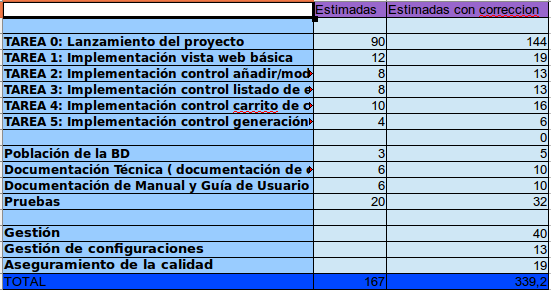
\includegraphics[width=0.95\textwidth]{img/6141}
\caption{Esfuerzos primera iteración}
 \label{fig:6141}
\end{figure}

\paragraph{} Se puede apreciar como la parte más importante de la primera iteración fue el lanzamiento, en el cual se planifico todo el proyecto para concretar todo e intentar evitar posibles problemas. Entre las demás partes se planifico que pruebas, gestión y implementación serías las siguientes tareas más costosas. Esto se puede ver en la~\cref{fig:6142}.

\begin{figure}[h!]
\centering
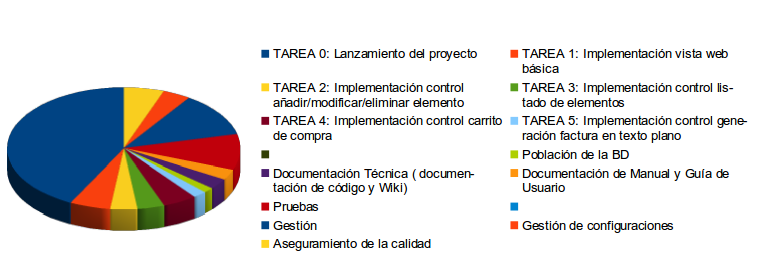
\includegraphics[width=0.95\textwidth]{img/6142}
\caption{Gráfica esfuerzos primera iteración}
 \label{fig:6142}
\end{figure}

\paragraph{} Se muestran los esfuerzos previstos para la segunda iteración del proyecto en la~\cref{fig:6143}. Podemos observar que la mayor parte de horas se la llevan la mejora de la implementación de la interfaz web (con la intención de que la misma tenga un aspecto llamativo y atractivo para el cliente) y las pruebas (con la intención de asegurar completamente que el producto que se le entrega al cliente funciona correctamente en su totalidad). Podemos ver dicho reparto de trabajo más claramente en la~\cref{fig:6144}. 

\begin{figure}[h!]
\centering
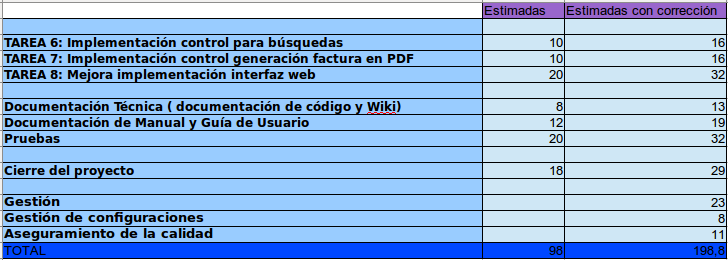
\includegraphics[width=0.95\textwidth]{img/6143}
\caption{Esfuerzos segunda iteración}
 \label{fig:6143}
\end{figure}

\begin{figure}[h!]
\centering
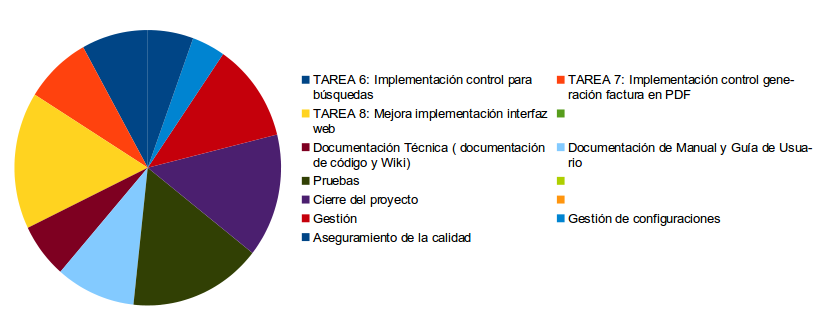
\includegraphics[width=0.95\textwidth]{img/6144}
\caption{Gráfica esfuerzos segunda iteración}
 \label{fig:6144}
\end{figure}
\blindtext
% 06.1.5
\subsubsection{Ficheros de esfuerzos individuales}
% 06.1.5. FICHEROS DE ESFUERZOS INDIVIDUALES 
%----------------------------------------------------------------------------------------

\blindtext
% 06.1.6
\subsubsection{Esfuerzos reales de las tareas}
% 06.1.6. ESFUERZOS REALES DE LAS TAREAS POR ITERACIÓN 
%----------------------------------------------------------------------------------------

\blindtext
% 06.1.7
\subsubsection{Esfuerzos reales de las personas}
% 06.1.7. ESFUERZOS REALES DE LAS PERSONAS Y ROLES 
%----------------------------------------------------------------------------------------

\paragraph{} Se muestran los datos y las gráficas con las horas realizadas por las diferentes personas del equipo en las figuras ~\cref{fig:6171} y ~\cref{fig:6172}. 

\paragraph{} Los roles de los miembros del grupo son los siguientes:
\begin{itemize}
\item Daniel $\Rightarrow$ Director de proyecto
\item Alberto $\Rightarrow$ Verificación y validación
\item Javier $\Rightarrow$ Gestor de configuraciones
\item Héctor $\Rightarrow$ Gestor de calidad
\item Simón $\Rightarrow$ Gestor de desarrollo
\item Alejandro $\Rightarrow$ Gestor de planificación
\end{itemize}

\paragraph{} En la gráfica ~\cref{fig:6171} se ven las diferentes horas invertidas por los integrantes del grupo. Daniel como director del proyecto invirtió el que más horas en el proyecto. Además el mes de Marzo fue en el que más horas se invirtieron.

\begin{figure}[h!]
\centering
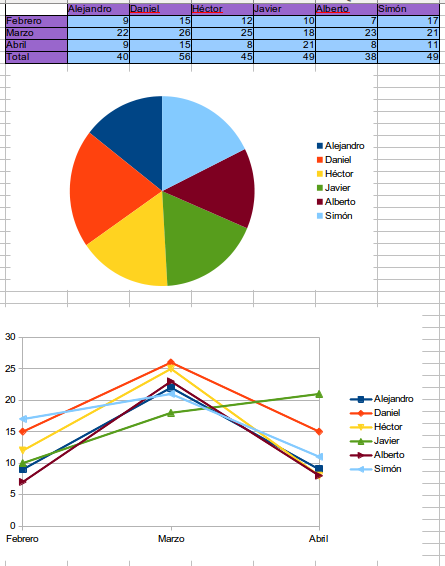
\includegraphics[width=0.95\textwidth]{img/6171}
\caption{Esfuerzos reales por persona primera iteración}
 \label{fig:6171}
\end{figure} 

\paragraph{} En cuanto a la segunda iteración también el director invirtió el que mas horas. Los demás integrantes del grupo más o menos hicieron las mismas horas.

\begin{figure}[h!]
\centering
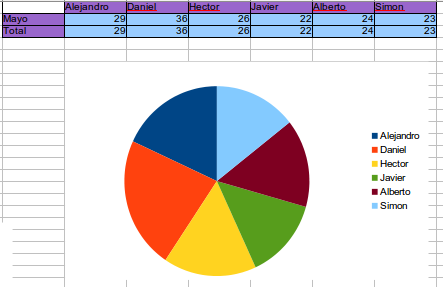
\includegraphics[width=0.95\textwidth]{img/6172}
\caption{Esfuerzos reales por persona primera iteración}
 \label{fig:6172}
\end{figure} 
\blindtext
% 06.2
\subsection{Procesos de seguimiento y control}
% 06.2. PROCESOS DE SEGUIMIENTO Y CONTROL
%----------------------------------------------------------------------------------------
Para el seguimiento y control de nuestro proyecto se han ido realizando reuniones de todo el grupo cada semana o cada dos semanas. En ellas se analizaba el trabajo realizado hasta ese momento, se planificaban y repartían nuevas tareas y se resolvían posibles dudas o problemas que pudieran surgir.
\blindtext
% 06.2.1
\subsubsection{Calendario de reuniones}
% 06.2.1. CALENDARIO DE LAS DISTINTAS REUNIONES CELEBRADAS
%----------------------------------------------------------------------------------------
\begin{itemize}
\item R-01 Lanzamiento de equipo: 	 20/02/2014 - 10:00
\item R-02 Lanzamiento de proyecto: 20/02/2014 - 12:00
\item R-03 Lanzamiento de proyecto: 26/02/2014 - 20:00
\item R-04 Seguimiento de proyecto y 1$^a$ iteración: 06/03/2014 - 10:00
\item R-05 Práctica 3, Comienzo primera iteración: 06/03/2014 - 12:00
\item R-06 Reunión de seguimiento semanal: 10/03/2014 - 20:00
\item R-07 Reunión interna de seguimiento: 12/03/2014 - 20:00 
\item R-08 Reunión de seguimiento: 27/03/2014 10:00
\item R-09 Reunión de organización para Aseguramiento de la Calidad del proyecto: 27/03/2014 -12:00
\item R-10 Reunión de seguimiento: 09/04/2014 -20:00
\item R-11 Reunión final de 1$^a$ iteración y comienzo de la 2$^a$: 09/04/2014 - 20:00
\end{itemize}

\blindtext
% 06.2.2
\subsubsection{Actas de reuniones}
% 06.2.2. ACTAS DE LAS DISTINTAS REUNIONES CELEBRADAS
%----------------------------------------------------------------------------------------
Se muestran a continuación los enlaces directos a las actas de cada una de las reuniones
\begin{itemize}
%\item R-01 Lanzamiento de equipo -- Anexo \ref{subsec:r1}
\item \reuniones{r01_lanzamiento_del_equipo/acta/r01_e20_acta}{R-01 Lanzamiento de equipo}
%\item R-02 Lanzamiento de proyecto -- Anexo \ref{subsec:r2}
\item \reuniones{r02_lanzamiento_del_proyecto/acta/r02_e20_acta}{R-02 Lanzamiento del proyecto}
%\item R-03 Lanzamiento de proyecto -- Anexo \ref{subsec:r3}
\item \reuniones{r03_lanzamiento_del_proyecto_cont/acta/r03_e20_acta}{R-03 Lanzamiento del proyecto II}
%\item R-04 Seguimiento de proyecto y 1$^a$ iteración -- Anexo \ref{subsec:r4}
\item \reuniones{r04_seguimiento_propuesta_proyecto/acta/r04_e20_acta}{R-04 Seguimiento de la propuesta de proyecto}
%\item R-05 Práctica 3, Comienzo primera iteración -- Anexo \ref{subsec:r5}
\item \reuniones{r05_comienzo_1a_iteracion/acta/r05_e7_acta}{R-05 Comienzo 1$^a$ iteración}
%\item R-06 Reunión de seguimiento semanal -- Anexo \ref{subsec:r6}
\item \reuniones{r06_reunion_seguimiento/acta/r06_e20_acta}{R-06 Reunión de seguimiento del proyecto}
%\item R-07 Reunión interna de seguimiento -- Anexo \ref{subsec:r7}
\item \reuniones{r07_reunion_seguimiento/acta/r07_e7_acta}{R-07 Reunión de seguimiento del proyecto}
%\item R-08 Reunión de seguimiento -- Anexo \ref{subsec:r8}
\item \reuniones{r08_reunion_seguimiento/acta/r08_e20_acta}{R-08 Reunión de seguimiento del proyecto}
%\item R-09 Reunión para Aseguramiento de la Calidad del proyecto -- Anexo \ref{subsec:r9}
\item \reuniones{r09_aseguramiento_calidad_proyecto/acta/r09_e20_acta}{R-09 Aseguramiento de calidad del proyecto}
%\item R-10 Reunión de seguimiento -- Anexo \ref{subsec:r10}
\item \reuniones{r10_reunion_seguimiento/acta/r10_e20_acta}{R-10 Reunión de seguimiento del proyecto}
%\item R-11 Reunión final de 1$^a$ iteración y comienzo de la 2$^a$ -- Anexo \ref{subsec:r11}
\item \reuniones{r11_final_1a_iteracion/acta/r11_e20_acta}{R-11 Reunión final de 1$^a$ iteración y comienzo de la 2$^a$}
\end{itemize}
\blindtext
% 06.3
\subsection{Coste}
% 06.3. COSTE REAL DEL PROYECTO
%----------------------------------------------------------------------------------------

\blindtext
%==============================================================================================
% 07.   GESTIÓN DE CONFIGURACIONES DEL PROYECTO
% 07.1. POLÍTICAS DE NOMBRADO
% 07.2. CONTROL DE VERSIONES
% 07.3. COPIAS DE SEGURIDAD
% 07.4. ELEMENTOS DE CONFIGURACIÓN Y LINEA BASE
%==============================================================================================

% 07
\section{Gestión de configuraciones}
% 07. GESTIÓN DE CONFIGURACIONES DEL PROYECTO
%==============================================================================================

\blindtext
% 07.1
\subsection{Políticas de nombrado}
% 07.1. POLÍTICAS DE NOMBRADO
%----------------------------------------------------------------------------------------------
El nombrado de ficheros debe realizarse en minúsculas, sin espacios, pudiendo utilizar en su caso el carácter '_'.

El nombre de cada fichero debe finalizar con una extensión separada del nombre del fichero por un punto, siendo la extensión en minúsculas y apropiada al tipo de contenido del fichero (php, png, html, txt, pdf...).
\blindtext
% 07.2
\subsection{Control de versiones}
% 07.2. CONTROL DE VERSIONES
%----------------------------------------------------------------------------------------------
El control de versiones utilizado será subversion, utilizándose como servicio de almacenamiento el de Google: Google Code, dada su elevada disponibilidad, siendo de esta manera accesible el proyecto para todos los miembros del equipo.

\blindtext
% 07.3
\subsection{Copias de seguridad}
% 07.3. COPIAS DE SEGURIDAD
%----------------------------------------------------------------------------------------------
Durante el desarrollo del proyecto se ha dispuesto en todo momento de una copia del sistema, operativa, a fin de poder llevar a cabo pruebas con el sistema online. Esta copia ha jugado un doble papel: el de servir como copia de seguridad en caso de no poder acceder a Google Code y el de servir como copia viva del entorno.
\blindtext
% 07.4
\subsection{Elementos de configuración y línea base}
% 07.4. ELEMENTOS DE CONFIGURACIÓN Y LINEA BASE
%----------------------------------------------------------------------------------------------

\blindtext
%==============================================================================================
% 08.   ASEGURAMIENTO DE LA CALIDAD DEL PROYECTO
% 08.1. ESTÁNDARES UTILIZADOS
% 08.2. PLANIFICACIÓN DE LAS AUDITORÍAS
% 08.3. AUDITORÍAS
% 08.4. AUDITORÍA EXTERNA
%==============================================================================================

% 08
\section{Aseguramiento de la calidad}
% 08. ASEGURAMIENTO DE LA CALIDAD DEL PROYECTO
%==============================================================================================
Para asegurar la calidad de nuestro proyecto nuestros objetivos han sido mejorar el software monitorizándolo apropiadamente y también el proceso de desarrollo que lo produce. 
De esta manera se busca asegurar la completa concordancia con los estándares y procedimientos establecidos para nuestro software y nuestro proceso de desarrollo.
Con ello conseguimos que cualquier elemento que no sea adecuado en el producto, el proceso, o los estándares es puesto en conocimiento de los responsables para que pueda ser resuelto.

\blindtext
% 08.1
\subsection{Estándares utilizados}
% 08.1. ESTÁNDARES UTILIZADOS
%----------------------------------------------------------------------------------------------
Como estándar utilizado a lo largo de todo el proceso se ha seguido una \textbf{guía de codificación} definida al principio del proyecto y de la cual no nos hemos apartado.
Se compone de las siguientes pautas:

\begin{itemize}
	\item Longitud máxima de línea recomendada, 80 carácteres.
	\item Métodos/funciones de un máximo recomendado de 30 líneas.
	\item Nombres de clase en mayúscula.
	\item Nombres de métodos/funciones en minúscula.
	\item Tabulado con dos espacios.
	\item Codificación UTF-8 en todos los ficheros de texto plano.
	\item Es importante respetar el indentado en el código fuente php/html "crudo" pero no se tratará de que el código esté correctamente indentado tras pasar por el intérprete php.
\end{itemize}









\blindtext
% 08.2
\subsection{Planificación de las auditorías}
% 08.2. PLANIFICACIÓN DE LAS AUDITORÍAS
%----------------------------------------------------------------------------------------------
\begin{itemize}
	\item La \textbf{auditoría interna} se planificó para el día 7 de Mayo de 2014 y se estimó una duración de 1 hora. Finalmente se llevó a cabo ese día pero la duración fue de 50 minutos.
	\item La \textbf{auditoría externa} se planificó para el día 9 de Mayo de 2014 y se estimó una duración de 1 hora. Finalmente se llevó a cabo ese día pero la duración fue de 80 minutos.
\end{itemize}
\blindtext
% 08.3
\subsection{Auditorías}
% 08.3. AUDITORÍAS
%----------------------------------------------------------------------------------------------
\newcommand{\audiInterna}[2]{\href{run:../../auditorias/interna/#1.xls}{#2}}
\paragraph{}Para el seguimiento de la calidad del equipo de desarrollo, se ha comprobado el seguimiento de las bases establecidas al inicio del proyecto con una herramienta clave como son las auditorías.
\paragraph{}Éste es el método principal para validar la calidad de un proceso o de un producto ya que realiza un examen de parte o todo de ese sistema y de su documentación para encontrar problemas potenciales.

\paragraph{}En el \audiInterna{auditoria_interna}{siguiente enlace} se puede encontrar la auditoría interna realizada a nuestro proyecto.
\blindtext
% 08.4
\subsection{Auditoría externa}
% 08.4. AUDITORÍA EXTERNA
%----------------------------------------------------------------------------------------------
\newcommand{\audiExterna}[2]{\href{run:../../auditorias/externa/#1.xls}{#2}}
\paragraph{}En el \audiExterna{auditoria_externa}{siguiente enlace} se puede encontrar la auditoría externa realizada a nuestro proyecto.
\blindtext
% 08.5
\subsection{No conformidades}
% 08.5. NO CONFORMIDADES
%----------------------------------------------------------------------------------------------

\blindtext
%==============================================================================================
% 09.   POSTMORTEM DEL PROYECTO
% 09.1. LECCIONES APRENDIDAS
% 09.2. PROBLEMAS ENCONTRADOS
% 09.3. CATÁLOGO DE RIESGOS
% 09.4. ANÁLISIS DIFERENCIAS ESFUERZOS Y TAMAÑOS REALES DEL PROYECTO VS LOS ESTIMADOS
% 09.5. PLAN REAL VS PLANIFICACIÓN INCIAL
% 09.6. ANÁLISIS DIFERENCIAS COSTE REAL DEL PROYECTO VS PRESUPUESTO
%==============================================================================================

% 09
\section{Postmortem}
% 09. POSTMORTEM DEL PROYECTO
%==============================================================================================

\blindtext
% 09.1
\subsection{Lecciones aprendidas}
% 09.1. LECCIONES APRENDIDAS
%----------------------------------------------------------------------------------------------
Se enumeran aquí alguna de las lecciones aprendidas por los miembros del equipo durante el desarrollo del proyecto:
\begin{itemize}
	\item Se ha aprendido la importancia del reparto de roles. Si bien la dimensión del proyecto no era quizás lo suficientemente grande para sacarle el máximo beneficio a esto, sí que sin este tipo de organización hubiera sido mucho más díficil llevar todo a cabo. Teniendo cada miembro un papel bien definido dentro del proyecto es mucho más fácil el realizar todas las tareas y juntar el trabajo periódicamente.
	\item A pesar de tener varios canales de comunicación entre los miembros del equipo (\textit{Whatsapp}, correo electrónico (\textit{Google Groups})...), es muy importante las reuniones periódicas para poner en común el trabajo. Es decir, en persona y cara a cara es mucho más efectivo trabajar, es muy importante para el desarrollo del proyecto.
	\item Se ha aprendido la importancia de buscar siempre varias alternativas a los problemas que surgen, poner ideas en común y llegar a un acuerdo como grupo. Por ejemplo, la decisión final de realizar el proyecto implementando la el catálogo con un \textit{Framework} como \textit{CodeIgniter} fue una decisión consensuada y finalmente vital para realizar a tiempo el proyecto. Así como la decisión de utilizar \textit{LaTex} para la documentación, decisión consensuada también y que ha agilizado mucho todo el desarrollo del proyecto.
	\item Se ha aprendido la importancia de que los miembros del equipo no sólo se ciñan a su papel, sino que también estén al día como mínimo de otros aspectos del proyecto. Pues si algún día faltaba un miembro o no estaba disponible durante algún tiempo, alguien tenía que suplirle temporalmente. De igual manera, es importante que el director esté al tanto de todo y se interese por el trabajo del resto de miembros del equipo.
	\item Se ha aprendido la importancia de planificar un proyecto antes de comenzarlo. Sí aún planificándolo ha habido momentos de cierta descordinación, sin la planificación pudiera haber sido un desastre que se ha evitado.
	\item Se ha aprendido la importancia de utilizar una herramienta de control de versiones como \textit{SubVersion} para desarrollo del proyecto, pudiendo deshacer cambios y errores, teniendo al instante los cambios realizados por otro compañero, etc. Además de aprender a utilizar este tipo de herramientas para futuros proyectos.
\end{itemize}
\paragraph{}En resumen, estás son algunas de las lecciones más importantes aprendidas, pero ha sido de gran importancia el aprender en general como trabajar en grupo con roles definidos y planificando cada aspecto de un proyecto.
\blindtext
% 09.2
\subsection{Problemas encontrados}
% 09.2. PROBLEMAS ENCONTRADOS
%----------------------------------------------------------------------------------------------
Se enumeran aquí algunos de los problemas que el equipo se ha ido encontrado durante el desarrollo del proyecto:

\begin{itemize}
	\item Aprendizaje para manejar el control de versiones de \textit{SubVersion}. Hubo problemas al inicio cuando había conflictos de modificación de ficheros.
	\item Aprendizaje de PHP por el resto de integrantes del equipo, pues sólo teníamos un experto en dicho lenguaje.
	\item Encontrar días y horas para realizar las reuniones y que todos los integrantes del equipo pudieran acudir.
\end{itemize}

\paragraph{} En general se podria decir que el proyecto se ha ido desarrollando sin muchos problemas. La mayoría de poca importancia y rápida solución, lo cual se puede considerar un punto a favor de la organización del equipo.

\blindtext
% 09.3
\subsection{Catálogo de riesgos}
% 09.3. CATÁLOGO DE RIESGOS
%----------------------------------------------------------------------------------------------

\blindtext
% 09.4
\subsection{Diferencias entre los esfuerzos y tamaños reales y los estimados}
% 09.4. ANÁLISIS DIFERENCIAS ESFUERZOS Y TAMAÑOS REALES DEL PROYECTO VS LOS ESTIMADOS
%----------------------------------------------------------------------------------------------
\paragraph{}Como se ha visto en el apartado \ref{sec:esfuerzos_reales} de este documento, en el desarrollo del proyecto en general el equipo ha realizado menos horas de esfuerzo de las estimadas en la planificación.

\paragraph{}Esto es debido principalmente a que el equipo ya contaba con experiencia anterior en otros proyectos de esta índole en el apartado de implementación y pruebas principalmente, con lo que al finalel trabajo se ha realizado quizás en estos apartados con mayor soltura de la esperada.

\paragraph{}Aún así, si nos fijamos en esas gráficas (~\cref{fig:6162} y ~\cref{fig:6164}) se puede comprobar que el total de horas reales empleadas se encuentra en un termino medio entre las estimadas y las estimadas con el factor de corrección aplicado. Es decir, que simplemente aplicando un factor de correción menor (igual fue demasiado alto por el miedo a quedarnos cortos y el desconocimiento de nunca haber realzado antes una planificación de este tipo) las horas estimadas y reales hubieran estado a un nivel muy similar. Por lo tanto, damos por satisfactorio la diferencia final entre dichas horas de esfuerzo y nos servirá para próximos proyectos.
\blindtext
% 09.5
\subsection{Plan real vs planificación inicial}
% 09.5. PLAN REAL VS PLANIFICACIÓN INCIAL
%----------------------------------------------------------------------------------------------

\blindtext
% 09.6
\subsection{Diferencias entre el coste real y el presupuesto}
% 09.6. ANÁLISIS DIFERENCIAS COSTE REAL DEL PROYECTO VS PRESUPUESTO
%----------------------------------------------------------------------------------------------
\paragraph{}Como ya se explica en el apartado \ref{subsec:coste} de este documento, y siguiendo el análisis de que las horas reales empleadas en el proyecto han sido menos que las estimadas inicialmente, pues evidentemente el coste real del proyecto es menor al estimado en el presupuesto. Esto daría como resultado final un beneficio a nuestra empresa de 8.388,62\euro, es decir, un resultado del que no nos podríamos quejar.

\paragraph{} De todas formas, esto también nos sirve para próximos proyectos regular el factor de correción aplicado al proyecto, quizás como ya se ha dicho antes, ha sido algo más elevado de lo que debiera, de ahí la diferencia económica a nuestro favor.
\blindtext
%==============================================================================================
% 10. CONCLUSIONES
% 10.1. CONCLUSIONES DEL PROYECTO
% 10.2. IDEAS DE MEJORA DEL PROCESO
% 10.3. IDEAS DE MEJORA DEL DESARROLLO DEL PROYECTO DENTRO DE LA ASIGNATURA
% 10.4. VALORACIONES SUBJETIVAS PERO ARGUMENTADAS
%==============================================================================================

% 10
\section{Conclusiones}
% 10. CONCLUSIONES
%==============================================================================================

\blindtext
% 10.1
\subsection{Conclusiones del proyecto}
% 10.1. CONCLUSIONES DEL PROYECTO
%----------------------------------------------------------------------------------------------

\blindtext
% 10.2
\subsection{Ideas de mejora del proceso}
% 10.2. IDEAS DE MEJORA DEL PROCESO
%----------------------------------------------------------------------------------------------

\blindtext
% 10.3
\subsection{Ideas de mejora del desarrollo del proyecto dentro de la asignatura}
% 10.3. IDEAS DE MEJORA DEL DESARROLLO DEL PROYECTO DENTRO DE LA ASIGNATURA
%----------------------------------------------------------------------------------------------

\blindtext
% 10.4
\subsection{Valoraciones subjetivas}
% 10.4. VALORACIONES SUBJETIVAS PERO ARGUMENTADAS
%----------------------------------------------------------------------------------------------
Como ya se ha dicho anteriormente, valoramos de forma bastante positiva el proyecto desarrolado en la asignatura, asi como la forma de trabajar que se nos ha impuesto/planteado para dicho desarrollo.

Se ha aprendido bastante en el aspecto de organización, planificación y trabajo en grupo; y no sólo aprendido, sino captado la importancia de ello en el desarrollo de un proyecto.

Personalmente, pensamos que hicimos una gran elección al decidir realizar un catálogo electrónico para la web alejándonos de la programación con \textit{Java GUI} o \textit{Android}, que seguramente hubieran complicado la implementación y nos hubiera quitado tiempo para el resto de apartados del proyecto.

Estamos además muy satisfechos con el rendimiento del equipo y con el hecho de que no hayan existido malos rollos ni problemas de esa índole, lo que ha facilitado mucho todo el desarrollo del proyecto. Valoramos también la ayuda del profesor Javier Zarazaga en las reuniones varias que se han realizado, y que con la dinámica que impone en ellas favorece ese buen trabajo en grupo que hemos tenido y el solucionar de la mejor manera posible todos los posibles problemas que iban surgiendo.

En resumen, una gran experiencia es la adquirida en este proyecto realizado y que estamos seguros en un futuro nos sirva como base para próximos proyectos en los que los diferentes miembros del equipo nos veamos involucrados.
\blindtext
%==============================================================================================
% ANEXOS
\appendix
%\addcontentsline{toc}{section}{ANEXOS}

%==============================================================================================
% A. CURRICULUMS VITAE
% A.1. CURRICULUM VITAE: DANIEL
% A.2. CURRICULUM VITAE: JAVIER
% A.3. CURRICULUM VITAE: JAVIER
% A.4. CURRICULUM VITAE: ALEJANDRO
% A.5. CURRICULUM VITAE: ALBERTO
% A.6. CURRICULUM VITAE: HÉCTOR
%==============================================================================================

% A
\section{Currículums Vitae}
% A. CURRICULUMS VITAE
%==============================================================================================


% A.1
\subsection{CV: Daniel García Páez}
% A.1. CURRICULUM VITAE: DANIEL
%----------------------------------------------------------------------------------------------
\begin{cv}{Curriculum Vitae}
	
\begin{cvlist}{Lenguajes de programación utilizados}
\item Conocimiento avanzado de Java
\item Conocimiento medio-avanzado de HTML,CSS,JSP,XML. Programación Web
\item Conocimiento deMySQL,SQL
\item Conocimiento medio de programación Android
\item Conocimiento medio de C
\item Conocimiento básico de PHP
\end{cvlist}

\begin{cvlist}{Experiencia}

	\item Realización de una aplicación web (HTML, CSS, JSP, XML) de red social.
	\item Realización de una aplicación web (HTML, CSS, JSP, XML) de operaciones con clientes y
cuentas bancarias.
	\item Creación y mantenimiento de varias bases de datos en MySQL.
	\item Realización de una aplicación móvil de gestión de notas para Android. Incluido todo el
proceso de análisis, requisitos, diseño e implementación del proyecto.

\end{cvlist}

\begin{cvlist}{Formación}

	\item[2008 a 2014] Estudiante de la EINA
		Grado en \textbf{Ingeniería informática} en la rama de \textbf{Software}\\
	\item[Inglés]  nivel avanzado(B2) de la escuela de Cambridge.


\end{cvlist}

\end{cv}

% A.2
\subsection{CV: Javier Briz Alastrué}
% A.2. CURRICULUM VITAE: JAVIER
%----------------------------------------------------------------------------------------------


% A.3
\subsection{CV: Simón Ortego Parra}
% A.3. CURRICULUM VITAE: SIMÓN
%----------------------------------------------------------------------------------------------
\begin{cv}{}
\vspace{2em}

\begin{cvlist}{Lenguajes de programación utilizados}
\item Java (+Android SDK), C
\item Ensamblador : ARM (+THUMB), SPARC, Intel, DLXV. OpenMP
\item Haskell, Erlang
\item Python, Ruby, sh
\item HTML, CSS, JSP, XML
\item SQL
\end{cvlist}

\begin{cvlist}{Experiencia}
	\item[Actualidad] Desarrollo de una aplicación Web para la conversión y 
	visualización de preparaciones histológicas virtuales utilizando pirámides 
	de imágenes (HTML, PHP y Javascript).

	\item[2012-actualidad] Creación y mantenimiento de varias bases de datos
	relacionales (Oracle y MySQL).
	
	\item[2013] Desarrollo de una aplicación Web de películas mediante el uso
	de HTML junto con JSPs y una base de datos MySQL.
	
	\item[2013] Realización de una aplicación móvil de gestión de notas para Android.

	\item[2012] Participación en un curso básico de Latex en la Asociación de Ingenieros 
	en Informática de Aragón.
	
\end{cvlist}

\begin{cvlist}{Formación}

	\item[2010 a 2014] Estudiante de la EINA
		Grado en \textbf{Ingeniería informática} en la rama de \textbf{Ingeniería de Computadores}\\
	\item[Inglés] Certificate in Advanced English (equiv. C1), de la universidad de Cambridge.
	\item[Alemán] Goethe-Zertifikat C1 (Zentrale MittelStufenPrüfung)
\end{cvlist}

\end{cv}

% A.4
\subsection{CV: Alejandro Gracia Mateo}
% A.4. CURRICULUM VITAE: ALEJANDRO
%----------------------------------------------------------------------------------------------


% A.5
\subsection{CV: Alberto Berbel Aznar}
% A.5. CURRICULUM VITAE: ALBERTO
%----------------------------------------------------------------------------------------------
\begin{cv}{Curriculum Vitae}

\begin{cvlist}{Lenguajes de programación utilizados}
\item Java, C, C++,(ensamblador)
\item ARM, ARM thumb
\item CLIPS, Haskell, erlang
\item HTML, CSS, JSP, XML
\item Matlab, SQL
\end{cvlist}

\begin{cvlist}{Experiencia}

	\item[2013] Realización de un Documento de Especificación de Requisitos 
				de un sistema real.
	
	\item[2013] Desarrollo de una nueva funcionalidad para un sistema de gran 
				tama\~no en lenguaje de programación Java.
	
	\item[2013] Herramientas de control de versiones como Bitbucket.
	
	\item[2013] Técnicas y herramientas de validación y verificación de software.
	
	\item[2013] Herramientas para la gestión y análisis de requisitos.
	
	\item[2013] Herramientas de seguimiento de errores como Bugzilla.
	
	\item[Actualidad] Desarrollo de una aplicación web consistente en un Smart Campus.

\end{cvlist}

\begin{cvlist}{Formación}

	\item[2010 a 2014] Estudiante de la EINA
		Grado en Ingeniería Informática en la especialidad de Ingeniería Software


\end{cvlist}

\end{cv}

% A.6
\subsection{CV: Héctor Francia Molinero}
% A.6. CURRICULUM VITAE: HÉCTOR
%----------------------------------------------------------------------------------------------
\begin{cv}{Curriculum Vitae}

\begin{cvlist}{Lenguajes de programación utilizados}
\item Ada, Java, C, C++, Android
\item Ensamblador, ARM, ARM thumb
\item CLIPS, Haskell, erlang
\item HTML, CSS, XML
\item Matlab, SQL
\end{cvlist}

\begin{cvlist}{Experiencia}

	\item[2011] Participación en la creación de una empresa de ocio.
	\item[2011] Creación de un programa para verificar documentos bien formados en XML con Flex y Bison
	\item[2012] Creación de un juego de dominó con programación concurrente.
	\item[2013] Realización de un compresor de ficheros de texto.
	\item[2013] Creación de una BD ``policial'' en MySQL.
	\item[2013] Realización de una aplicación móvil de gestión de notas para Android.
	\item[2013] Realización de una página de recomendación de películas.
	\item[2013] Realización de un sistema de chat para múltiples usuarios con Erlang y Java.
	\item[2013] Realización de un compilador para un lenguaje similar a MiniLang.
	\item[2013] Creación de una página Web usando el CMS Wordpress.

\end{cvlist}

\begin{cvlist}{Formación}

	\item[2008 a 2011] Estudiante de \textbf{Ingeniería Superior informática}
	\item[2011 a 2014] Estudiante de la EINA
		Grado en \textbf{Ingeniería informática} en la rama de \textbf{computación}


\end{cvlist}

\end{cv}

%==============================================================================================
% B. HOJAS DE ESFUERZOS
% B.1. HOJA DE ESFUERZOS: DANIEL
% B.1. HOJA DE ESFUERZOS: DANIEL
% B.2. HOJA DE ESFUERZOS: JAVIER
% B.3. HOJA DE ESFUERZOS: SIMÓN
% B.4. HOJA DE ESFUERZOS: ALEJANDRO
% B.5. HOJA DE ESFUERZOS: ALBERTO
% B.6. HOJA DE ESFUERZOS: HÉCTOR
%==============================================================================================

% B
\section{Hojas de esfuerzos}
%% B. HOJAS DE ESFUERZOS
%==============================================================================================

%\blindtext
% B.1
\subsection{Hoja de esfuerzos: Daniel García Páez}
%% B.1. HOJA DE ESFUERZOS: DANIEL
%----------------------------------------------------------------------------------------------

En el \hojaesfuerzos{b_1_hoja_de_esfuerzos_daniel}{siguiente enlace} se puede acceder a la hoja de 
esfuerzos de Daniel.

% B.2
\subsection{Hoja de esfuerzos: Javier Briz Alastrué}
%% B.2. HOJA DE ESFUERZOS: JAVIER
%----------------------------------------------------------------------------------------------

En el \hojaesfuerzos{b_2_hoja_de_esfuerzos_javier}{siguiente enlace} se puede acceder a la hoja de 
esfuerzos de Javier.

% B.3
\subsection{Hoja de esfuerzos: Simón Ortego Parra}
%% B.3. HOJA DE ESFUERZOS: SIMÓN
%----------------------------------------------------------------------------------------------

En el \hojaesfuerzos{b_3_hoja_de_esfuerzos_simon}{siguiente enlace} se puede acceder a la hoja de 
esfuerzos de Simón.

% B.4
\subsection{Hoja de esfuerzos: Alejandro Gracia Mateo}
%% B.4. HOJA DE ESFUERZOS: ALEJANDRO
%----------------------------------------------------------------------------------------------

En el \hojaesfuerzos{b_4_hoja_de_esfuerzos_alejandro}{siguiente enlace} se puede acceder a la hoja de 
esfuerzos de Alejandro.

% B.5
\subsection{Hoja de esfuerzos: Alberto Berbel Aznar}
%% B.5. HOJA DE ESFUERZOS: ALBERTO
%----------------------------------------------------------------------------------------------

En el \hojaesfuerzos{b_5_hoja_de_esfuerzos_alberto}{siguiente enlace} se puede acceder a la hoja de 
esfuerzos de Alberto.

% B.6
\subsection{Hoja de esfuerzos: Héctor Francia Molinero}
%% B.6. HOJA DE ESFUERZOS: HÉCTOR
%----------------------------------------------------------------------------------------------

En el \hojaesfuerzos{b_6_hoja_de_esfuerzos_hector}{siguiente enlace} se puede acceder a la hoja de 
esfuerzos de Héctor.

%==============================================================================================
% C. CRONOGRAMAS
% C.1. CRONOGRAMA INICIAL
% C.2. CRONOGRAMA FINAL
%==============================================================================================

% C
\section{Cronogramas}
% C. CRONOGRAMAS
%==============================================================================================

\blindtext
% C.1
\subsection{Cronograma inicial}
% C.1. CRONOGRAMA INICIAL
%----------------------------------------------------------------------------------------------

\blindtext
% C.2
\subsection{Cronograma final}
% C.2. CRONOGRAMA FINAL
%----------------------------------------------------------------------------------------------

\blindtext
%==============================================================================================
% D.    ACTAS DE REUNIONES
% D.01. ACTA DE REUNION #01
% D.02. ACTA DE REUNION #02
% D.03. ACTA DE REUNION #03
% D.04. ACTA DE REUNION #04
% D.05. ACTA DE REUNION #05
% D.06. ACTA DE REUNION #06
% D.07. ACTA DE REUNION #07
% D.08. ACTA DE REUNION #08
% D.10. ACTA DE REUNION #10
% D.11. ACTA DE REUNION #11
% D.12. ACTA DE REUNION #12
%==============================================================================================

% D
\section{Actas de reuniones}
% D. ACTAS DE REUNIONES
%==============================================================================================
\begin{itemize}
%\item R-01 Lanzamiento de equipo -- Anexo \ref{subsec:r1}
\item \reuniones{r01_lanzamiento_del_equipo/acta/r01_e20_acta}{R-01 Lanzamiento de equipo}
%\item R-02 Lanzamiento de proyecto -- Anexo \ref{subsec:r2}
\item \reuniones{r02_lanzamiento_del_proyecto/acta/r02_e20_acta}{R-02 Lanzamiento del proyecto}
%\item R-03 Lanzamiento de proyecto -- Anexo \ref{subsec:r3}
\item \reuniones{r03_lanzamiento_del_proyecto_cont/acta/r03_e20_acta}{R-03 Lanzamiento del proyecto II}
%\item R-04 Seguimiento de proyecto y 1$^a$ iteración -- Anexo \ref{subsec:r4}
\item \reuniones{r04_seguimiento_propuesta_proyecto/acta/r04_e20_acta}{R-04 Seguimiento de la propuesta de proyecto}
%\item R-05 Práctica 3, Comienzo primera iteración -- Anexo \ref{subsec:r5}
\item \reuniones{r05_comienzo_1a_iteracion/acta/r05_e7_acta}{R-05 Comienzo 1$^a$ iteración}
%\item R-06 Reunión de seguimiento semanal -- Anexo \ref{subsec:r6}
\item \reuniones{r06_reunion_seguimiento/acta/r06_e20_acta}{R-06 Reunión de seguimiento del proyecto}
%\item R-07 Reunión interna de seguimiento -- Anexo \ref{subsec:r7}
\item \reuniones{r07_reunion_seguimiento/acta/r07_e7_acta}{R-07 Reunión de seguimiento del proyecto}
%\item R-08 Reunión de seguimiento -- Anexo \ref{subsec:r8}
\item \reuniones{r08_reunion_seguimiento/acta/r08_e20_acta}{R-08 Reunión de seguimiento del proyecto}
%\item R-09 Reunión para Aseguramiento de la Calidad del proyecto -- Anexo \ref{subsec:r9}
\item \reuniones{r09_aseguramiento_calidad_proyecto/acta/r09_e20_acta}{R-09 Aseguramiento de calidad del proyecto}
%\item R-10 Reunión de seguimiento -- Anexo \ref{subsec:r10}
\item \reuniones{r10_reunion_seguimiento/acta/r10_e20_acta}{R-10 Reunión de seguimiento del proyecto}
%\item R-11 Reunión final de 1$^a$ iteración y comienzo de la 2$^a$ -- Anexo \ref{subsec:r11}
\item \reuniones{r11_final_1a_iteracion/acta/r11_e20_acta}{R-11 Reunión final de 1$^a$ iteración y comienzo de la 2$^a$}
\end{itemize}

% D.1
\subsection{Reunión núm.01}
% D.01. ACTA DE REUNION #01
%----------------------------------------------------------------------------------------------
\begin{center}	
\Large{Acta de Reunión Nº \numeroDeReunion\hspace{0.25em}-\hspace{0.25em}\tituloReunion}
\end{center}
\vspace{1.5em}

% PRIMERA TABLA: INFORMACIÓN BÁSICA
\begin{longtable}{ | L{\dimexpr 0.420\linewidth-2\tabcolsep} |
				     L{\dimexpr 0.570\linewidth-2\tabcolsep} | }
\hline % ------------------------------------------------------------------------
\rowcolor{grisCabeceraTabla}
\mc{2}{\bf Información básica}  \\
%\hline % ------------------------------------------------------------------------
%{\bf Cliente} & Nombre del cliente (por definir o no es necesario ?)  \\
\hline % ------------------------------------------------------------------------
{\bf Proyecto} & $\mu$Search \\ 
\hline % ------------------------------------------------------------------------
{\bf Fecha y hora de comienzo} & 20/02/14 - 12:00 \\
\hline % ------------------------------------------------------------------------
{\bf Lugar} & Seminario 21, Edif. Ada Byron. EINA. Unizar \\
\hline % ------------------------------------------------------------------------
{\bf Tipo de reunión} & Estándar \\
\hline % ------------------------------------------------------------------------
\end{longtable}


%----------------------------------------------------------------------------------------
% SEGUNDA TABLA - ASISTENTES
\begin{longtable}{ | C{\dimexpr 0.070\linewidth-2\tabcolsep} |
                     L{\dimexpr 0.350\linewidth-2\tabcolsep} |
                     C{\dimexpr 0.370\linewidth-2\tabcolsep} |
                     C{\dimexpr 0.200\linewidth-2\tabcolsep} | }
\hline % ------------------------------------------------------------------------
\rowcolor{grisCabeceraTabla}
\mc{4}{\bf Asistentes} \\
\hline % ------------------------------------------------------------------------
{\bf Nº} & {\bf Nombre y Apellidos} & {\bf Cargo} & {\bf Rol} \\
\hline % ------------------------------------------------------------------------
{\bf 1} & Alberto Berbel Aznar & Verificación y validación & --  \\
\hline % ------------------------------------------------------------------------
{\bf 2} & Javier Briz Alastrué & Gestor de configuraciones & --  \\
\hline % ------------------------------------------------------------------------
{\bf 3} & Héctor Francia Molinero & Gestor de calidad & --  \\
\hline % ----------------------------------------------------
{\bf 4} & Daniel García Páez & Director del proyecto & -- \\
\hline % ------------------------------------------------------------------------
{\bf 5} & Alejandro Gracia Mateo & Gestor de planificación & --  \\
\hline % ------------------------------------------------------------------------
{\bf 6} & Simón Ortego Parra & Gestor de desarrollo & Secretario  \\
\hline % ------------------------------------------------------------------------
{\bf 7} & Fco. Javier Zarazaga Soria & -- & Preparador  \\
\hline % ------------------------------------------------------------------------
\end{longtable}

%----------------------------------------------------------------------------------------
% CUARTA TABLA - OBJETIVOS, CUERPO DE LA REUNIÓN, DECISIONES TOMADAS, ...
\begin{longtable}{ | C{\dimexpr\linewidth-2\tabcolsep} | }
\hline % ------------------------------------------------------------------------
\cabeceraTabla{Objetivos} \\
\hline % ------------------------------------------------------------------------
\endfirsthead
\hline % ------------------------------------------------------------------------
\endhead
\espacioSubtabla
\hline % ------------------------------------------------------------------------
\endfoot
\hline % ------------------------------------------------------------------------
\endlastfoot

\itemNvlUno{Establecer las políticas y aspectos de organización generales comunes
para un buen funcionamiento de equipo.}\\

\hline % ------------------------------------------------------------------------
\cabeceraTabla{Cuerpo de la reunión} \\
\hline % ------------------------------------------------------------------------
\itemNvlUno{Previamente a realizar la reunión (sin el profesor) se decidieron
algunos aspectos organizativos.}
\itemNvlUno{Se decidió la asignación definitva de los roles los miembros del grupo 
para el proyecto, tal y como se muestra en la parte superior del acta.}
\itemNvlUno{Se establecieron algunos aspectos de la política de reuniones:}
	\itemNvlDos{Los roles de director, secretario y planificador serán fijos para todas 
	las reuniones.}
	\itemNvlDos{Los roles de cronometrador y observador serán rotados entre los tres 
	miembros restantes del grupo, quedando así siempre un miembro libre de rol que nos 
	podrá venir bien para el caso de que algún miembro no pueda acudir a alguna reunión.}
	\itemNvlDos{Día y hora de las reuniones de seguimiento periódicas: Miércoles a las 20:00h}
\itemNvlUno{Se establecieron algunas políticas a seguir en situaciones conflictivas:}
	\itemNvlDos{Si algún miembro llega tarde a una reunión, dar comienzo a la misma 
	sin su presencia.}
	\itemNvlDos{La toma de decisiones serán conjunta. Se escucharán las argumentaciones 
	de cada miembro y se realizará una votación.}	
\itemNvlUno{Cuando comenzó la reunión, cada uno de los asistentes se presentó a la hora.}	
\itemNvlUno{Cada uno de los asistentes planteó brevemente su vida y experiencias en 
general, y lo relacionado al desarrollo de software en particular.}
\itemNvlUno{El profesor asistente planteó de manera detallada y general en que suele 
consistir el desarrollo de un proyecto software de pequeña escala y los aspectos 
importantes a considerar en el desarrollo de este proyecto.}
\itemNvlUno{El profesor asistente especificó la manera en que debiera presentarse 
la propuesta del proyecto software.}
\itemNvlUno{Se decidió fijar como cliente a una tienda de venta de 
microcontroladores, de tal forma que estuviese muy acotada la solución, y a
su vez se plantease como muy sencilla.}
\itemNvlUno{Se recordaron los requisitos solicitados de la aplicación por los
profesores de la asignatura.}
\itemNvlUno{Tras recalcar el profesor los requisitos no funcionales especificados,
se decidió que la aplicación fuera desarrollada como una aplicación Web utilizando 
para ello las tecnologías PHP, MySQL y CodeIgniter.}
\itemNvlUno{Se realizó una foto del equipo.}\\

\pagebreak
\hline % ------------------------------------------------------------------------
\cabeceraTabla{Decisiones tomadas}  \\
\hline % ------------------------------------------------------------------------

\itemNvlUno{Se ha decidido que el catálogo electrónico de la tienda fuese una 
sobre la venta de microcontroladores.}
\itemNvlUno{Se establecen como tecnologías para el desarrollo de la aplicación PHP,
MySQL y CodeIgniter.}\\

\hline % ------------------------------------------------------------------------
\cabeceraTabla{Temas pendientes} \\
\hline % ------------------------------------------------------------------------

\itemNvlUno{Rotular la fotografía del equipo para que los profesores de la asignatura
puedan así identificar mejor a los componentes del equipo.}\\

\cabeceraTabla{Próxima reunión prevista} \\
\hline % ------------------------------------------------------------------------
Jueves 06 de Marzo del 2014 a las 10:00 
\end{longtable}

% D.2
\subsection{Reunión núm.02}
% D.02. ACTA DE REUNION #02
%----------------------------------------------------------------------------------------------
\begin{center}	
\Large{Acta de Reunión Nº02\hspace{0.25em}-\hspace{0.25em}\tituloReunion}
\end{center}
\vspace{1.5em}

% PRIMERA TABLA: INFORMACIÓN BÁSICA
\begin{longtable}{ | L{\dimexpr 0.420\linewidth-2\tabcolsep} |
				     L{\dimexpr 0.570\linewidth-2\tabcolsep} | }
\hline % ------------------------------------------------------------------------
\rowcolor{grisCabeceraTabla}
\mc{2}{\bf Información básica}  \\
%\hline % ------------------------------------------------------------------------
%{\bf Cliente} & Nombre del cliente (por definir o no es necesario ?)  \\
\hline % ------------------------------------------------------------------------
{\bf Proyecto} & $\mu$Search \\ 
\hline % ------------------------------------------------------------------------
{\bf Fecha y hora de comienzo} & 20/02/14 - 12:00 \\
\hline % ------------------------------------------------------------------------
{\bf Lugar} & Seminario 21, Edif. Ada Byron. EINA. Unizar \\
\hline % ------------------------------------------------------------------------
{\bf Tipo de reunión} & Estándar \\
\hline % ------------------------------------------------------------------------
\end{longtable}


%----------------------------------------------------------------------------------------
% SEGUNDA TABLA - ASISTENTES
\begin{longtable}{ | C{\dimexpr 0.070\linewidth-2\tabcolsep} |
                     L{\dimexpr 0.350\linewidth-2\tabcolsep} |
                     C{\dimexpr 0.370\linewidth-2\tabcolsep} |
                     C{\dimexpr 0.200\linewidth-2\tabcolsep} | }
\hline % ------------------------------------------------------------------------
\rowcolor{grisCabeceraTabla}
\mc{4}{\bf Asistentes} \\
\hline % ------------------------------------------------------------------------
{\bf Nº} & {\bf Nombre y Apellidos} & {\bf Cargo} & {\bf Rol} \\
\hline % ------------------------------------------------------------------------
{\bf 1} & Alberto Berbel Aznar & Verificación y validación & --  \\
\hline % ------------------------------------------------------------------------
{\bf 2} & Javier Briz Alastrué & Gestor de configuraciones & --  \\
\hline % ------------------------------------------------------------------------
{\bf 3} & Héctor Francia Molinero & Gestor de calidad & --  \\
\hline % ----------------------------------------------------
{\bf 4} & Daniel García Páez & Director del proyecto & -- \\
\hline % ------------------------------------------------------------------------
{\bf 5} & Alejandro Gracia Mateo & Gestor de planificación & --  \\
\hline % ------------------------------------------------------------------------
{\bf 6} & Simón Ortego Parra & Gestor de desarrollo & Secretario  \\
\hline % ------------------------------------------------------------------------
\end{longtable}

%----------------------------------------------------------------------------------------
% CUARTA TABLA - OBJETIVOS, CUERPO DE LA REUNIÓN, DECISIONES TOMADAS, ...
\begin{longtable}{ | C{\dimexpr\linewidth-2\tabcolsep} | }
\hline % ------------------------------------------------------------------------
\cabeceraTabla{Objetivos} \\
\hline % ------------------------------------------------------------------------
\endfirsthead
\hline % ------------------------------------------------------------------------
\endhead
\espacioSubtabla
\hline % ------------------------------------------------------------------------
\endfoot
\hline % ------------------------------------------------------------------------
\endlastfoot

\itemNvlUno{Organizar de forma consensuada el comienzo del proyecto y algunos
aspectos generales.} \\

\hline % ------------------------------------------------------------------------
\cabeceraTabla{Cuerpo de la reunión} \\
\hline % ------------------------------------------------------------------------

\itemNvlUno{Cada uno de los asistentes se presentó a la hora.}
\itemNvlUno{Se analizaron los requisitos de la aplicación de nuevo y
se fijaron perfectamente todos los parámetros.}
\itemNvlUno{Se pasó a hablar de la arquitectura en alto nivel del sistema
a desarrollar y de realizar los diagramas explicativos apropiados (diagramas
de componentes y de despliegue).}
\itemNvlUno{Se establecieron las tecnologías y estándares de codificación del
proyecto software.}
\itemNvlUno{Se decidieron las herramientas usadas para la documentación durante 
el desarrrollo del proyecto.}
\itemNvlUno{Se establecieron los mecanismos de comunicación entre los componentes
del equipo.}
\itemNvlUno{Se realizó una planificación de las tareas ha realizar inmediatamente
para el desarrollo del documento de ``Propuesta de Proyecto''.}\\

\hline % ------------------------------------------------------------------------
\cabeceraTabla{Decisiones tomadas}  \\
\hline % ------------------------------------------------------------------------

\itemNvlUno{Se establecieron como tecnologías y estándares de codificación (los
establecidos por los desarrolladores de éstas) las siguientes:}
	\itemNvlDos{HTML 5.}
	\itemNvlDos{CSS 3.}
	\itemNvlDos{PHP 5 y CodeIgniter (la versión apropiada).}
	\itemNvlDos{MySQL.}
	\itemNvlDos{LaTex: para la generación de la órden de pedido automática.}
\itemNvlUno{Para la documentación durante el desarrrollo del proyecto
se van a utilizar las siguientes herramientas:}
	\itemNvlDos{LaTex: para todo tipo de documentación (Actas, Convocatorias...)}
	\itemNvlDos{Excel o similar: para la anotación de los esfuerzos
	de los miembros del equipo.}
	\itemNvlDos{Modelio: para realizar diferentes diagramas de la arquitectura del software.}
	\itemNvlDos{Subversion: para el almacenamiento de todos los documentos.}
\itemNvlUno{Para la comunicación entre los miembros se van a utilizar:}
	\itemNvlDos{Google Groups: para todo tipo de comunicación.}
	\itemNvlDos{Whatsapp: para la comunicación informal (problemas, retrasos, citas,...)}
\itemNvlUno{Se realizó la siguiente planificación de cara a la presentación de la
``Propuesta de Proyecto'' que incluye una aproximación del número de horas y
los miembros a los que se les asigna cada una de las tareas:}
	\itemNvlDos{[2 h.] - Diagrama E/R de la BD + prototipo de la 
	aplicación en papel: Daniel y Javier.}
	\itemNvlDos{[1 h.] - Diseño arquitectural del sistema (diag. componentes 
	y despliegue): Alberto.}
	\itemNvlDos{[1 h.] - Plantillas de documentación en LaTeX para las actas,
	convocatorias y propuesta de proyecto: Simón.}
	\itemNvlDos{[1 h.] - Hojas de esfuerzos: Códigos de categorías (incluyendo un 
	documento de texto explicativo con código + nombre + descr.): Alejandro}
	\itemNvlDos{[2 h.] - Logotipo + Nombre de la empresa: Héctor.}\\

\hline % ------------------------------------------------------------------------
\cabeceraTabla{Temas pendientes} \\
\hline % ------------------------------------------------------------------------

\itemNvlUno{Elección del responsable de la propuesta de proyecto.}
\itemNvlUno{Calendario de trabajo.}
\itemNvlUno{Iniciar el uso de la Wiki + Subversion.} \\
	
\hline % ------------------------------------------------------------------------
\cabeceraTabla{Próxima reunión prevista} \\
\hline % ------------------------------------------------------------------------
Miércoles 26 de Febrero del 2014 a las 20:00 \\
\end{longtable}


% D.3
\subsection{Reunión núm.03}
% D.03. ACTA DE REUNION #03
%----------------------------------------------------------------------------------------------


% D.4
\subsection{Reunión núm.04}
% D.04. ACTA DE REUNION #04
%----------------------------------------------------------------------------------------------	
\begin{center}	
\Large{Acta de Reunión Nº04\hspace{0.25em}-\hspace{0.25em}\tituloReunion}
\end{center}
\vspace{1.5em}

% PRIMERA TABLA: INFORMACIÓN BÁSICA
\begin{longtable}{ | L{\dimexpr 0.420\linewidth-2\tabcolsep} |
				     L{\dimexpr 0.570\linewidth-2\tabcolsep} | }
\hline % ------------------------------------------------------------------------
\rowcolor{grisCabeceraTabla}
\mc{2}{\bf Información básica}  \\
%\hline % ------------------------------------------------------------------------
%{\bf Cliente} & Nombre del cliente (por definir o no es necesario ?)  \\
\hline % ------------------------------------------------------------------------
{\bf Proyecto} & $\mu$Search \\
\hline % ------------------------------------------------------------------------
{\bf Fecha y hora de reunión} & 06/03/14 - 10:00 \\
\hline % ------------------------------------------------------------------------
{\bf Lugar} & Seminario 25, Edif. Ada Byron. EINA. Unizar \\
\hline % ------------------------------------------------------------------------
{\bf Tipo de reunión} & Reunión TP6 con Profesor \\
\hline % ------------------------------------------------------------------------
\end{longtable}


%----------------------------------------------------------------------------------------
% SEGUNDA TABLA - ASISTENTES
\begin{longtable}{ | C{\dimexpr 0.070\linewidth-2\tabcolsep} |
                     L{\dimexpr 0.350\linewidth-2\tabcolsep} |
                     C{\dimexpr 0.370\linewidth-2\tabcolsep} |
                     C{\dimexpr 0.200\linewidth-2\tabcolsep} | }
\hline % ------------------------------------------------------------------------
\rowcolor{grisCabeceraTabla}
\mc{4}{\bf Asistentes} \\
\hline % ------------------------------------------------------------------------
{\bf Nº} & {\bf Nombre y Apellidos} & {\bf Cargo} & {\bf Rol} \\
\hline % ------------------------------------------------------------------------
{\bf 1} & Alberto Berbel Aznar & Verificación y validación & --  \\
\hline % ------------------------------------------------------------------------
{\bf 2} & Javier Briz Alastrué & Gestor de configuraciones & --  \\
\hline % ------------------------------------------------------------------------
{\bf 3} & Héctor Francia Molinero & Gestor de calidad & --  \\
\hline % ----------------------------------------------------
{\bf 4} & Daniel García Páez & Director del proyecto & -- \\
\hline % ------------------------------------------------------------------------
{\bf 5} & Alejandro Gracia Mateo & Gestor de planificación & --  \\
\hline % ------------------------------------------------------------------------
{\bf 6} & Simón Ortego Parra & Gestor de desarrollo & Secretario  \\
\hline % ------------------------------------------------------------------------
{\bf 7} & Fco. Javier Zaragaza Soria & -- & Preparador  \\
\hline % ------------------------------------------------------------------------
\end{longtable}

%----------------------------------------------------------------------------------------
% CUARTA TABLA - OBJETIVOS, CUERPO DE LA REUNIÓN, DECISIONES TOMADAS, ...
\begin{longtable}{ | C{\dimexpr\linewidth-2\tabcolsep} | }
\hline % ------------------------------------------------------------------------
\rowcolor{grisCabeceraTabla}
{\bf Objetivos} \\
\hline % ------------------------------------------------------------------------
\endfirsthead
\hline % ------------------------------------------------------------------------
\endhead
\espacioSubtabla
\hline % ------------------------------------------------------------------------
\endfoot
\hline % ------------------------------------------------------------------------
\endlastfoot

\itemNvlUno{El objetivo principal de está reunion es el de realizar un seguimiento, con el profesor preparador Fco. Javier Zaragza, de nuestra propuesta de proyecto y de como se está abordando la primera iteración del proyecto software a realizar para su lanzamiento para poder ir cerrando y concretando varios apartados.}\\

% ------------------------------------------------------------------------
\rowcolor{grisCabeceraTabla}
{\bf Cuerpo de la reunión} \\
\hline % ------------------------------------------------------------------------

\itemNvlUno{Cada uno de los asistentes se presentó a la hora.}
\itemNvlUno{El equipo pusó al día al preparador sobre el avance en la propuesta de proyecto, todo aquello que ya estaba decidido. }
\itemNvlUno{El preparador nos ofreció varios consejos y pautas para la modificación y mejora de los requisitos que habíamos establecido en reuniones previas.}
\itemNvlUno{Se pasó a discutir ampliamente con el preparador para recibir su consejo sobre dos de los aspectos más complicados de abordar de la propuesta de proyecto:}
\itemNvlDos{Planificación de la 1ª iteración del proyecto en tareas y asignación de horas aproximadas a cada tarea. Que diferentes técnicas se pueden seguir para realizar la aproximación.}
\itemNvlDos{Realización de la oferta de presupuesto del proyecto.}
\itemNvlUno{Por último, se negoció la fijación de fechas para:}
\itemNvlDos{Siguiente reunión de seguimiento de la primera iteración.}
\itemNvlDos{Lanzamiento de la segunda iteración.}
\\

\hline % ------------------------------------------------------------------------
\rowcolor{grisCabeceraTabla}
{\bf Decisiones tomadas}  \\
\hline % ------------------------------------------------------------------------

\itemNvlUno{Se decidió que había que mejorar y detallar ciertos aspectos de los requisitos del sistema:}
\itemNvlDos{La definición de elemento: microcontrolador caracterizado por nº de referencia, arquitectura, flash, memoria, ...}
\itemNvlDos{Establecer en base a que característica de los microcontroladores se mostrarán ordenados los listados de búsqueda.}
\itemNvlDos{Establecer los datos personales que el cliente deberá rellenar a la hora de pedir la generación de una factura.}
\itemNvlDos{En caso de existir alguna restricción o limitación sobre el sistema o plataforma de desarrollo del proyecto software, añadirlas como requisitos no funcionales.}
\itemNvlUno{Se decide que la división de tareas tanto para la planificación como para el presupuesto se realizará en base a los requisitos establecidos.}
\itemNvlUno{Se incluirá una primera actividad o tarea denominada como "Tarea 0" que será el lanzamiento del proyecto, incluyendo la estructura inicial del proyecto: zona de arranque, instalación del SGBD, creación de la BD...}
\itemNvlUno{Se decidió la no utilización de máquinas virtuales para trabajar en el mismo entorno. Cada miembro trabajará en su propio equipo con las versiones de las tecnologías (PHP, MySQL, HTML...) a utilizar ya establecidas.}
\itemNvlUno{Se decide modificar la hoja de esfuerzos proporcionada en clase, de forma que todas las tareas que cada miembro del equipo haga irán incluida en una de la siguientes tareas:}
\itemNvlDos{Tareas ligadas a los requisitos.}
\itemNvlDos{Documentación.}
\itemNvlDos{Pruebas.}
\itemNvlDos{Reuniones técnicas y no técnicas (o de planificación).}
\\

\hline % ------------------------------------------------------------------------
\rowcolor{grisCabeceraTabla}
{\bf Temas pendientes} \\
\hline % ------------------------------------------------------------------------

\itemNvlUno{Establecimiento de las fechas de:}
\itemNvlDos{Reunión de seguimiento de la primera iteración.}
\itemNvlDos{Fecha de lanzamiento de la segunda iteración.}
\itemNvlUno{Modificación final de los requisitos del sistema para la propuesta de proyecto.}
\itemNvlUno{Especificación de las tareas en las que se dividirá la planificación del proyecto y realización de la oferta de presupuesto a partir de las misma.}
\\

\hline % ------------------------------------------------------------------------
\rowcolor{grisCabeceraTabla}
{\bf Próxima reunión prevista} \\
\hline % ------------------------------------------------------------------------
Reunión semanal  12/03/2014 20:00
\end{longtable}



% D.5
\subsection{Reunión núm.05}
% D.05. ACTA DE REUNION #05
%----------------------------------------------------------------------------------------------s	
\begin{center}	
\Large{Acta de Reunión Nº05\hspace{0.25em}-\hspace{0.25em}\tituloReunion}
\end{center}
\vspace{0.8em}

% PRIMERA TABLA: INFORMACIÓN BÁSICA
\begin{longtable}{ | L{\dimexpr 0.420\linewidth-2\tabcolsep} |
				     L{\dimexpr 0.570\linewidth-2\tabcolsep} | }
\hline % ------------------------------------------------------------------------
\rowcolor{grisCabeceraTabla}
\mc{2}{\bf Información básica}  \\
%\hline % ------------------------------------------------------------------------
%{\bf Cliente} & Nombre del cliente (por definir o no es necesario ?)  \\
\hline % ------------------------------------------------------------------------
{\bf Proyecto} & $\mu$Search \\ 
\hline % ------------------------------------------------------------------------
{\bf Fecha y hora de comienzo} & 06/03/14 - 12:00 \\
\hline % ------------------------------------------------------------------------
{\bf Lugar} & Seminario 21, Edif. Ada Byron. EINA. Unizar \\
\hline % ------------------------------------------------------------------------
{\bf Tipo de reunión} & Estándar \\
\hline % ------------------------------------------------------------------------
\end{longtable}


%----------------------------------------------------------------------------------------
% SEGUNDA TABLA - ASISTENTES
\begin{longtable}{ | C{\dimexpr 0.070\linewidth-2\tabcolsep} |
                     L{\dimexpr 0.350\linewidth-2\tabcolsep} |
                     C{\dimexpr 0.370\linewidth-2\tabcolsep} |
                     C{\dimexpr 0.200\linewidth-2\tabcolsep} | }
\hline % ------------------------------------------------------------------------
\rowcolor{grisCabeceraTabla}
\mc{4}{\bf Asistentes} \\
\hline % ------------------------------------------------------------------------
{\bf Nº} & {\bf Nombre y Apellidos} & {\bf Cargo} & {\bf Rol} \\
\hline % ------------------------------------------------------------------------
{\bf 1} & Alberto Berbel Aznar & Verificación y validación & --  \\
\hline % ------------------------------------------------------------------------
{\bf 2} & Javier Briz Alastrué & Gestor de configuraciones & Cronometrador  \\
\hline % ------------------------------------------------------------------------
{\bf 3} & Héctor Francia Molinero & Gestor de calidad & Observador  \\
\hline % ----------------------------------------------------
{\bf 4} & Daniel García Páez & Director del proyecto & Director \\
\hline % ------------------------------------------------------------------------
{\bf 5} & Alejandro Gracia Mateo & Gestor de planificación & --  \\
\hline % ------------------------------------------------------------------------
{\bf 6} & Simón Ortego Parra & Gestor de desarrollo & Secretario  \\
\hline % ------------------------------------------------------------------------
\end{longtable}

%----------------------------------------------------------------------------------------
% CUARTA TABLA - OBJETIVOS, CUERPO DE LA REUNIÓN, DECISIONES TOMADAS, ...
\begin{longtable}{ | C{\dimexpr\linewidth-2\tabcolsep} | }
\hline % ------------------------------------------------------------------------
\rowcolor{grisCabeceraTabla}
{\bf Objetivos} \\
\hline % ------------------------------------------------------------------------
\endfirsthead
\hline % ------------------------------------------------------------------------
\endhead
\espacioSubtabla
\hline % ------------------------------------------------------------------------
\endfoot
\hline % ------------------------------------------------------------------------
\endlastfoot

\itemNvlUno{Postmortem de la propuesta de proyecto: analizar el funcionamiento del 
equipo durante la fase previa de realización de la propuesta de proyecto.}
\itemNvlUno{Lanzamiento de la primera iteración del proyecto.}\\

\hline % ------------------------------------------------------------------------
\rowcolor{grisCabeceraTabla}
{\bf Cuerpo de la reunión} \\
\hline % ------------------------------------------------------------------------

\itemNvlUno{Cada uno de los asistentes se presentaron a la hora.}
\itemNvlUno{Cada uno de los miembros del equipo comentaron el número de horas que llevan trabajadas en el proyecto.}
\itemNvlUno{Se revisó el trabajo compartido y se propusieron ideas para mejorar su gestión.}
\itemNvlUno{Se acordaron tecnologías y herramientas necesarias para el desarrollo del proyecto.}
\itemNvlUno{Se refinaron los requisitos establecidos en reuniones anteriores y se definieron nuevos requisitos.}
\itemNvlUno{Se fijaron las tareas a abordar durante la primera iteración del proyecto.}
\itemNvlUno{Se estableció el orden en el que serán abordados los requisitos.}
\itemNvlUno{Se realizó una estimación conjunta de los esfuerzos de cada tarea.}
\itemNvlUno{Comentarios finales de las conclusiones obtenidas.}\\

\hline % ------------------------------------------------------------------------
\rowcolor{grisCabeceraTabla}
{\bf Decisiones tomadas}  \\
\hline % ------------------------------------------------------------------------

\itemNvlUno{Cada uno de los miembros del grupo tendrá relativa libertad para elegir el entorno
  de desarrollo siempre y cuando lo codificado sea un fichero de texto (UTF-8) y funcione en la máquina destinada a pruebas:} 
  \itemNvlDos{ \emph{MySQL} (mysql ver 14.14 Distrib 5.5.35, for 	debian-linux-gnu)}
  \itemNvlDos{\emph{Apache} (Apache/2.2.22 (Debian))}
  \itemNvlDos{\emph{PHP} (PHP 5.4.4-14+deb7u7)}
		  
\itemNvlUno{Es necesario realizar ''commits'' muy frecuentemente para evitar conflictos o minimizarlos.}
\itemNvlUno{Nueva codificación de los ficheros compartidos: todos los nombres en minúsculas y sin espacios, utilizar underscores para separar las palabras.}  
\itemNvlUno{Se utilizará la Wiki para todo tipo de documentación.}
\itemNvlUno{Los requisitos de la aplicación a desarrollar son:}
\itemNvlDos{Un microcontrolador (elemento) estará compuesto de los siguientes campos: Referencia única para cada elemento, Arquitectura, Frecuencia, Flash, RAM y precio.}
\itemNvlDos{Insertar un nuevo elemento en el carro de compra.}
\itemNvlDos{Eliminar un elemento del carro de compra.}
\itemNvlDos{Modificar la cantidad solicitada de un elemento del carro de compra.}
\itemNvlDos{Se podrá acceder a los elementos del catálogo mediante un listado en el que aparezcan todos los elementos que se encuentren en el catálogo.}
\itemNvlDos{Se permitirá realizar la búsqueda de productos en cada caso en función de un único campo de búsqueda.}
\itemNvlDos{Los resultados de la búsqueda se presentarán de la siguiente forma: Un listado (sin paginación) que muestre de cada elemento todos sus campos en columnas.}
\itemNvlDos{Se permitirá realizar pedidos que incluirán los datos del cliente cada vez. Es decir, no existirá persistencia de los datos del cliente tras realizar pedidos. Los pedidos contendrán la suficiente información para identificar a los clientes. Además, no permitirán la reserva de los productos solicitados, únicamente generarán un presupuesto del coste de los productos elegidos.}
\itemNvlDos{Los datos solicitados del cliente para los pedidos son los siguientes: Nombre, Apellidos, Dirección, Ciudad, Provincia, País, Código postal, Teléfono, Mail. Además CIF y Empresa aparecerán como campos opcionales que servirán de distinción entre particulares y entidades.}
\itemNvlDos{Se añadirá una vista diferente para la administración del catálogo a la que no podrán acceder los clientes y se ejecutará localmente.}
\itemNvlDos{La administración del catálogo permitirá insertar un elemento en el catálogo a partir de las arquitecturas disponibles.}
\itemNvlDos{La administración del catálogo permitirá eliminar un elemento del catálogo.}
\itemNvlDos{La administración del catálogo permitirá modificar un elemento del catálogo.} 

\itemNvlUno{Tareas que se abordarán en la primera iteración:}
\itemNvlDos{\emph{Tarea 0}: Instalación. Desarrollo de la aplicación base (diseño de MVC, objetos, plataforma), sin interfaz Web.}
\itemNvlDos{\emph{Tarea 1}: Marco común de las páginas web.}
\itemNvlDos{\emph{Tarea 2}: Insertar, modificar y eliminar elementos.}
\itemNvlDos{\emph{Tarea 3}: Mostrar el listado completo de los elementos del catálogo.}
\itemNvlDos{\emph{Tarea 4}: Gestión de pedidos, primera versión sin generar PDF, en texto plano.}
\itemNvlDos{\emph{Tarea 5}: Gestión del carrito de compra.}
\itemNvlDos{Desarrollo progresivo de la interfaz web (vista de la aplicación).}

\itemNvlUno{Estimación conjunta de esfuerzos (horas por persona trabajando en la tarea):}
\itemNvlDos{Tarea 0: 2 horas.}
\itemNvlDos{Tarea 1: 1-2 horas.}
\itemNvlDos{Tarea 2: 4 horas.}
\itemNvlDos{Tarea 3: 2 horas.}
\itemNvlDos{Tarea 4: 5 horas.}
\itemNvlDos{Tarea 5: 5 horas.}

\itemNvlUno{Los encargados de desarrollar la parte del modelo del sistema (patrón MVC) son: Javier y Simón.}
\itemNvlUno{Los encargados de desarrollar la parte de la vista del sistema (patrón MVC) son: Daniel, Alejandro, Héctor y Alberto.}

\itemNvlUno{El producto final será un servicio que incluirá: la página web, el servidor web (Apache), la base de datos, el sistema de gestión de la base de datos.}\\

\hline % ------------------------------------------------------------------------
\rowcolor{grisCabeceraTabla}
{\bf Temas pendientes} \\
\hline % ------------------------------------------------------------------------

\itemNvlUno{Finalización del presupuesto.}
\itemNvlUno{Finalización de planificación de tareas para el proyecto.}
\itemNvlUno{Finalización de la propuesta del proyecto.} \\

\hline % ------------------------------------------------------------------------
\rowcolor{grisCabeceraTabla}
{\bf Próxima reunión prevista} \\
\hline % ------------------------------------------------------------------------
Lunes 10 de Marzo de 2014 a las 20:00  \\
\end{longtable}


% D.6
%\subsection{Reunión núm.06}
%% D.06. ACTA DE REUNION #06
%----------------------------------------------------------------------------------------------
\begin{center}	
\Large{Acta de Reunión Nº06\hspace{0.25em}-\hspace{0.25em}\tituloReunion}
\end{center}
\vspace{1.5em}

% PRIMERA TABLA: INFORMACIÓN BÁSICA
\begin{longtable}{ | L{\dimexpr 0.420\linewidth-2\tabcolsep} |
				     L{\dimexpr 0.570\linewidth-2\tabcolsep} | }
\hline % ------------------------------------------------------------------------
\rowcolor{grisCabeceraTabla}
\mc{2}{\bf Información básica}  \\
%\hline % ------------------------------------------------------------------------
%{\bf Cliente} & Nombre del cliente (por definir o no es necesario ?)  \\
\hline % ------------------------------------------------------------------------
{\bf Proyecto} & $\mu$Search \\
\hline % ------------------------------------------------------------------------
{\bf Fecha y hora de reunión} & 10/03/14 - 20:00 \\
\hline % ------------------------------------------------------------------------
{\bf Lugar} & Sala Informática A1, Edif. Ada Byron. EINA. Unizar \\
\hline % ------------------------------------------------------------------------
{\bf Tipo de reunión} & Estándar \\
\hline % ------------------------------------------------------------------------
\end{longtable}


%----------------------------------------------------------------------------------------
% SEGUNDA TABLA - ASISTENTES
\begin{longtable}{ | C{\dimexpr 0.070\linewidth-2\tabcolsep} |
                     L{\dimexpr 0.350\linewidth-2\tabcolsep} |
                     C{\dimexpr 0.370\linewidth-2\tabcolsep} |
                     C{\dimexpr 0.200\linewidth-2\tabcolsep} | }
\hline % ------------------------------------------------------------------------
\rowcolor{grisCabeceraTabla}
\mc{4}{\bf Asistentes} \\
\hline % ------------------------------------------------------------------------
{\bf Nº} & {\bf Nombre y Apellidos} & {\bf Cargo} & {\bf Rol} \\
\hline % ------------------------------------------------------------------------
{\bf 1} & Alberto Berbel Aznar & Verificación y validación & --  \\
\hline % ------------------------------------------------------------------------
{\bf 2} & Javier Briz Alastrué & Gestor de configuraciones & --  \\
\hline % ------------------------------------------------------------------------
{\bf 3} & Héctor Francia Molinero & Gestor de calidad & --  \\
\hline % ----------------------------------------------------
{\bf 4} & Daniel García Páez & Director del proyecto & -- \\
\hline % ------------------------------------------------------------------------
{\bf 5} & Alejandro Gracia Mateo & Gestor de planificación & --  \\
\hline % ------------------------------------------------------------------------
{\bf 6} & Simón Ortego Parra & Gestor de desarrollo & Secretario  \\
\hline % ------------------------------------------------------------------------
{\bf 7} & Fco. Javier Zaragaza Soria & -- & Preparador  \\
\hline % ------------------------------------------------------------------------
\end{longtable}

%----------------------------------------------------------------------------------------
% CUARTA TABLA - OBJETIVOS, CUERPO DE LA REUNIÓN, DECISIONES TOMADAS, ...
\begin{longtable}{ | C{\dimexpr\linewidth-2\tabcolsep} | }
\hline % ------------------------------------------------------------------------
\rowcolor{grisCabeceraTabla}
{\bf Objetivos} \\
\hline % ------------------------------------------------------------------------
\endfirsthead
\hline % ------------------------------------------------------------------------
\endhead
\espacioSubtabla
\hline % ------------------------------------------------------------------------
\endfoot
\hline % ------------------------------------------------------------------------
\endlastfoot
\itemNvlUno{El objetivo principal de está reunion es la definición y el reparto de las 
tareas a realizar para la propuesta de proyecto.}\\
% ------------------------------------------------------------------------
\rowcolor{grisCabeceraTabla}
{\bf Cuerpo de la reunión} \\
\hline % ------------------------------------------------------------------------

\itemNvlUno{Cada uno de los asistentes se presentó a la hora.}
\itemNvlUno{Se revisó brevemente la agenda de la reunión.}
\itemNvlUno{Se plantearon algunos aspectos relacionados con la gestión
de configuraciones.}
\itemNvlUno{Se realizó la división de las tareas para la propuesta de proyecto.}
\hline % ------------------------------------------------------------------------
\rowcolor{grisCabeceraTabla}
{\bf Decisiones tomadas}  \\
\hline % ------------------------------------------------------------------------
\itemNvlUno{Las siguientes fueron las tareas definidas a realizar para la propuesta de proyecto:}
    \itemNvlDos{Tarea 0:}
        \itemNvlTres{Requisitos + Análisis + Diseño.}
        \itemNvlTres{Instalación.}
        \itemNvlTres{Desarrollo de la aplicación base (diseño de MVC, objetos, 
        plataforma), sin interfaz Web (Vista).}
    \itemNvlDos{Tarea 1A:}
        \itemNvlTres{Marco común de la Web.}
    \itemNvlDos{Tarea 1B:}
        \itemNvlTres{Insertar + Modificar + Eliminar (máx 2 personas).}
    \itemNvlDos{Tarea 2:}
        \itemNvlTres{Mostrar el listado completo.}
    \itemNvlDos{Tarea 3:}
        \itemNvlTres{Gestión de pedidos.}
    \itemNvlDos{Tarea 4A:}
        \itemNvlTres{Documentación.}
    \itemNvlDos{Tarea 4B:}
        \itemNvlTres{Manuales.}\\
\hline % ------------------------------------------------------------------------
\rowcolor{grisCabeceraTabla}
{\bf Próxima reunión prevista} \\
\hline % ------------------------------------------------------------------------
Miércoles 12 de Marzo del 2014 a las 20:00
\end{longtable}

% D.7
\subsection{Reunión núm.07}
% D.07. ACTA DE REUNION #07
%----------------------------------------------------------------------------------------------
\begin{center}	
\Large{Acta de Reunión Nº07\hspace{0.25em}-\hspace{0.25em}\tituloReunion}
\end{center}
\vspace{1.5em}

% PRIMERA TABLA: INFORMACIÓN BÁSICA
\begin{longtable}{ | L{\dimexpr 0.420\linewidth-2\tabcolsep} |
				     L{\dimexpr 0.570\linewidth-2\tabcolsep} | }
\hline % ------------------------------------------------------------------------
\rowcolor{grisCabeceraTabla}
\mc{2}{\bf Información básica}  \\
%\hline % ------------------------------------------------------------------------
%{\bf Cliente} & Nombre del cliente (por definir o no es necesario ?)  \\
\hline % ------------------------------------------------------------------------
{\bf Proyecto} & $\mu$Search \\ 
\hline % ------------------------------------------------------------------------
{\bf Fecha y hora de comienzo} & 12/03/14 - 20:00 \\
\hline % ------------------------------------------------------------------------
{\bf Lugar} & Aula 3, Edif. Ada Byron. EINA. Unizar \\
\hline % ------------------------------------------------------------------------
{\bf Tipo de reunión} & Estándar \\
\hline % ------------------------------------------------------------------------
\end{longtable}


%----------------------------------------------------------------------------------------
% SEGUNDA TABLA - ASISTENTES
\begin{longtable}{ | C{\dimexpr 0.070\linewidth-2\tabcolsep} |
                     L{\dimexpr 0.350\linewidth-2\tabcolsep} |
                     C{\dimexpr 0.370\linewidth-2\tabcolsep} |
                     C{\dimexpr 0.200\linewidth-2\tabcolsep} | }
\hline % ------------------------------------------------------------------------
\rowcolor{grisCabeceraTabla}
\mc{4}{\bf Asistentes} \\
\hline % ------------------------------------------------------------------------
{\bf Nº} & {\bf Nombre y Apellidos} & {\bf Cargo} & {\bf Rol} \\
\hline % ------------------------------------------------------------------------
{\bf 1} & Alberto Berbel Aznar & Verificación y validación & Secretario  \\
\hline % ------------------------------------------------------------------------
{\bf 2} & Javier Briz Alastrué & Gestor de configuraciones & Cronometrador  \\
\hline % ------------------------------------------------------------------------
{\bf 3} & Héctor Francia Molinero & Gestor de calidad & Observador  \\
\hline % ----------------------------------------------------
{\bf 4} & Daniel García Páez & Director del proyecto & Director \\
\hline % ------------------------------------------------------------------------
{\bf 5} & Alejandro Gracia Mateo & Gestor de planificación & Planificador  \\
\hline %  ------------------------------------------------------------------------
\end{longtable}


%----------------------------------------------------------------------------------------
% TERCERA TABLA - AUSENTES
\begin{longtable}{ | C{\dimexpr 0.070\linewidth-2\tabcolsep} |
                     L{\dimexpr 0.350\linewidth-2\tabcolsep}  |
                     C{\dimexpr 0.570\linewidth-2\tabcolsep} | }
\hline % ------------------------------------------------------------------------
\rowcolor{grisCabeceraTabla}
\mc{3}{\bf Ausentes} \\ 
\hline % ------------------------------------------------------------------------
{\bf Nº} & {\bf Nombre y Apellidos} & {\bf Cargo} \\
\hline % ------------------------------------------------------------------------
{\bf 1} & Simón Ortego Parra & Gestor de desarrollo \\
\hline % ------------------------------------------------------------------------
\end{longtable}


%----------------------------------------------------------------------------------------
% CUARTA TABLA - OBJETIVOS, CUERPO DE LA REUNIÓN, DECISIONES TOMADAS, ...
\begin{longtable}{ | C{\dimexpr\linewidth-2\tabcolsep} | }
\hline % ------------------------------------------------------------------------
\rowcolor{grisCabeceraTabla}
{\bf Objetivos} \\
\hline % ------------------------------------------------------------------------
\endfirsthead
\hline % ------------------------------------------------------------------------
\endhead
\espacioSubtabla
\hline % ------------------------------------------------------------------------
\endfoot
\hline % ------------------------------------------------------------------------
\endlastfoot

\itemNvlUno{Revisión del trabajo realizado.}
\itemNvlUno{Elaboración de la propuesta del proyecto.}\\

\hline % ------------------------------------------------------------------------
\rowcolor{grisCabeceraTabla}
{\bf Cuerpo de la reunión} \\
\hline % ------------------------------------------------------------------------

\itemNvlUno{Simón Ortego Parra se ausentó por causa justificada.}
\itemNvlUno{Se revisó el trabajo realizado por cada componente del equipo.}
\itemNvlUno{Se elaboró el cronograma del primer ciclo.}
\itemNvlUno{Se elaboró el presupuesto del proyecto.}\\

\hline % ------------------------------------------------------------------------
\rowcolor{grisCabeceraTabla}
{\bf Decisiones tomadas}  \\
\hline % ------------------------------------------------------------------------

\itemNvlUno{Para la reunión de seguimiento deberíamos tener:}
\itemNvlDos{Al final de la primera semana: Tarea 1 y población de la base de datos.}
\itemNvlDos{De forma paralela las tareas 2, 3 y 4.}
\itemNvlUno{La reunión de seguimiento con Fco. Javier Zarazaga Soria, en principio, se establece el Jueves 27 de Marzo.} 
\itemNvlUno{La documentación técnica deberá estar acabada el día 10 de Abril.}
\itemNvlUno{La documentación de manuales se realizará desde el 10 de Abril, hasta el 24 de Abril.}
\itemNvlUno{Paralelamente a la realización de la documentación, se realizará la preparación de las pruebas (desde el 27 de Marzo hasta el 24 de abril).}
\itemNvlUno{A las pruebas se le asigna una carga de trabajo del 50\% de lo que cuesta implementar el código.}
\itemNvlUno{A la documentación se le asigna una carga de trabajo del 20\% de lo que cuesta implementar el código.}\\

\hline % ------------------------------------------------------------------------
\rowcolor{grisCabeceraTabla}
{\bf Temas pendientes} \\
\hline % ------------------------------------------------------------------------

\itemNvlUno{Finalizar propuesta del proyecto.} 
\itemNvlUno{Entregar en moodle actas pendientes.}\\

\hline % ------------------------------------------------------------------------
\rowcolor{grisCabeceraTabla}
{\bf Próxima reunión prevista} \\
\hline % ------------------------------------------------------------------------
Sin fijar (de momento)
\end{longtable}



% D.8
\subsection{Reunión núm.08}
% D.08. ACTA DE REUNION #08
%----------------------------------------------------------------------------------------------
\begin{center}	
\Large{Acta de Reunión Nº \numeroDeReunion\hspace{0.25em}-\hspace{0.25em}\tituloReunion}
\end{center}
\vspace{1.5em}

% PRIMERA TABLA: INFORMACIÓN BÁSICA
\begin{longtable}{ | L{\dimexpr 0.420\linewidth-2\tabcolsep} |
				     L{\dimexpr 0.570\linewidth-2\tabcolsep} | }
\hline % ------------------------------------------------------------------------
\rowcolor{grisCabeceraTabla}
\mc{2}{\bf Información básica}  \\
%\hline % ------------------------------------------------------------------------
%{\bf Cliente} & Nombre del cliente (por definir o no es necesario ?)  \\
\hline % ------------------------------------------------------------------------
{\bf Proyecto} & $\mu$Search \\ 
\hline % ------------------------------------------------------------------------
{\bf Fecha y hora de comienzo} & 27/03/14 - 10:00 \\
\hline % ------------------------------------------------------------------------
{\bf Lugar} & Seminario 21, Edif. Ada Byron. EINA. Unizar \\
\hline % ------------------------------------------------------------------------
{\bf Tipo de reunión} & Estándar \\
\hline % ------------------------------------------------------------------------
\end{longtable}


%----------------------------------------------------------------------------------------
% SEGUNDA TABLA - ASISTENTES
\begin{longtable}{ | C{\dimexpr 0.070\linewidth-2\tabcolsep} |
                     L{\dimexpr 0.350\linewidth-2\tabcolsep} |
                     C{\dimexpr 0.370\linewidth-2\tabcolsep} |
                     C{\dimexpr 0.200\linewidth-2\tabcolsep} | }
\hline % ------------------------------------------------------------------------
\rowcolor{grisCabeceraTabla}
\mc{4}{\bf Asistentes} \\
\hline % ------------------------------------------------------------------------
{\bf Nº} & {\bf Nombre y Apellidos} & {\bf Cargo} & {\bf Rol} \\
\hline % ------------------------------------------------------------------------
{\bf 1} & Alberto Berbel Aznar & Verificación y validación & --  \\
%\hline % ------------------------------------------------------------------------
%{\bf 2} & Javier Briz Alastrué & Gestor de configuraciones & --  \\
\hline % ------------------------------------------------------------------------
{\bf 3} & Héctor Francia Molinero & Gestor de calidad & --  \\
\hline % ----------------------------------------------------
{\bf 4} & Daniel García Páez & Director del proyecto & -- \\
\hline % ------------------------------------------------------------------------
{\bf 5} & Alejandro Gracia Mateo & Gestor de planificación & --  \\
\hline % ------------------------------------------------------------------------
{\bf 6} & Simón Ortego Parra & Gestor de desarrollo & Secretario  \\
\hline % ------------------------------------------------------------------------
\end{longtable}


%----------------------------------------------------------------------------------------
% TERCERA TABLA - AUSENTES
\begin{longtable}{ | C{\dimexpr 0.070\linewidth-2\tabcolsep} |
                     L{\dimexpr 0.350\linewidth-2\tabcolsep}  |
                     C{\dimexpr 0.570\linewidth-2\tabcolsep} | }
\hline % ------------------------------------------------------------------------
\rowcolor{grisCabeceraTabla}
\mc{3}{\bf Ausentes} \\ 
\hline % ------------------------------------------------------------------------
{\bf 1} & Javier Briz Alastrué & Gestor de configuraciones \\
\hline % ------------------------------------------------------------------------
\end{longtable}


%----------------------------------------------------------------------------------------
% CUARTA TABLA - OBJETIVOS, CUERPO DE LA REUNIÓN, DECISIONES TOMADAS, ...
\begin{longtable}{ | C{\dimexpr\linewidth-2\tabcolsep} | }
\hline % ------------------------------------------------------------------------
\rowcolor{grisCabeceraTabla}
{\bf Cuerpo de la reunión} \\
\hline % ------------------------------------------------------------------------
\endfirsthead
\hline % ------------------------------------------------------------------------
\endhead
\espacioSubtabla
\hline % ------------------------------------------------------------------------
\endfoot
\hline % ------------------------------------------------------------------------
\endlastfoot
\itemNvlUno{Cada uno de los asistentes se presentó a la hora.}

\itemNvlUno{El profesor asistente realizó una serie de preguntas
a los integrantes del equipo:}

	\itemNvlDos{En primer lugar, preguntó sobre el número de horas que
	habían sido dedicadas al proyecto y si se había realizado una estimación
	del porcentaje del proyecto que se llevaba desarrollado. La respuesta
	del equipo fue que no se había realizado dicha estimación, pero que
	aparecía en las hojas de esfuerzos individuales el número de horas
	dedicadas. El profesor también aconsejo que se realizase esta
	estimación no todas las semanas, pero sí siempre antes de una
	reunión de éste carácter.}

	\itemNvlDos{La segunda pregunta que planteó fue si había ocurrido
	o se estaban tratando con alguna dificultad en el desarrollo. El equipo
	respondió negativamente, y así se finalizó una parte importante de la
	reunión que estaba planteada para resolver cualquier problema que 
	pudiera haber ocurrido.}

\itemNvlUno{Los miembros del equipo le plantearon la fecha de entrega
de la primera iteración del proyecto, a lo que el profesor añadió que
era importante no olvidar realizar una estimación apropiada de las pruebas
y fijarlas en el calendario, teniendo en cuenta también que en la segunda
iteración solía ocurrir que había menos tiempo semanalmente para la 
dedicación al proyecto. A continuación, el profesor aconsejó realizar
una plantilla (estándar) para la realización de las pruebas y que era
un buen consejo que no realizara las pruebas la misma persona que 
había realizado la parte del código pertinente.}

\itemNvlUno{Como último aspecto importante el profesor recordó
que había que realizar las auditorías (una externa, realizada
por otro grupo, además de otra interna, como mínimo) y realizar
la planificación y el ajuste del calendario en base a éstas.}

\itemNvlUno{Por último se planteó una fecha para la siguiente reunión,
que podría cambiar si le venía mal a alguno de los convocados.}\\

\hline % ------------------------------------------------------------------------
\rowcolor{grisCabeceraTabla}
{\bf Próxima reunión prevista} \\
\hline % ------------------------------------------------------------------------
Viernes 09 de Mayo del 2014 a las 12:00 \\
\end{longtable}


% D.9
\subsection{Reunión núm.09}
% D.01. ACTA DE REUNION #09
%----------------------------------------------------------------------------------------------
\begin{center}	
\Large{Acta de Reunión Nº \numeroDeReunion\hspace{0.25em}-\hspace{0.25em}\tituloReunion}
\end{center}
\vspace{1.5em}

% PRIMERA TABLA: INFORMACIÓN BÁSICA
\begin{longtable}{ | L{\dimexpr 0.420\linewidth-2\tabcolsep} |
				     L{\dimexpr 0.570\linewidth-2\tabcolsep} | }
\hline % ------------------------------------------------------------------------
\rowcolor{grisCabeceraTabla}
\mc{2}{\bf Información básica}  \\
%\hline % ------------------------------------------------------------------------
%{\bf Cliente} & Nombre del cliente (por definir o no es necesario ?)  \\
\hline % ------------------------------------------------------------------------
{\bf Proyecto} & $\mu$Search \\ 
\hline % ------------------------------------------------------------------------
{\bf Fecha y hora de comienzo} & 20/02/14 - 12:00 \\
\hline % ------------------------------------------------------------------------
{\bf Lugar} & Seminario 21, Edif. Ada Byron. EINA. Unizar \\
\hline % ------------------------------------------------------------------------
{\bf Tipo de reunión} & Estándar \\
\hline % ------------------------------------------------------------------------
\end{longtable}


%----------------------------------------------------------------------------------------
% SEGUNDA TABLA - ASISTENTES
\begin{longtable}{ | C{\dimexpr 0.070\linewidth-2\tabcolsep} |
                     L{\dimexpr 0.350\linewidth-2\tabcolsep} |
                     C{\dimexpr 0.370\linewidth-2\tabcolsep} |
                     C{\dimexpr 0.200\linewidth-2\tabcolsep} | }
\hline % ------------------------------------------------------------------------
\rowcolor{grisCabeceraTabla}
\mc{4}{\bf Asistentes} \\
\hline % ------------------------------------------------------------------------
{\bf Nº} & {\bf Nombre y Apellidos} & {\bf Cargo} & {\bf Rol} \\
\hline % ------------------------------------------------------------------------
{\bf 1} & Alberto Berbel Aznar & Verificación y validación & Planificador \\
\hline % ------------------------------------------------------------------------
{\bf 2} & Javier Briz Alastrué & Gestor de configuraciones & Observador \\
\hline % ------------------------------------------------------------------------
{\bf 3} & Héctor Francia Molinero & Gestor de calidad & Director \\
\hline % ----------------------------------------------------
{\bf 4} & Daniel García Páez & Director del proyecto & Cronometrador \\
\hline % ------------------------------------------------------------------------
%{\bf 5} & Alejandro Gracia Mateo & Gestor de planificación & --  \\
%\hline % ------------------------------------------------------------------------
{\bf 6} & Simón Ortego Parra & Gestor de desarrollo & Secretario  \\
\hline % ------------------------------------------------------------------------
\end{longtable}


%----------------------------------------------------------------------------------------
% TERCERA TABLA - AUSENTES
\begin{longtable}{ | C{\dimexpr 0.070\linewidth-2\tabcolsep} |
                     L{\dimexpr 0.350\linewidth-2\tabcolsep}  |
                     C{\dimexpr 0.570\linewidth-2\tabcolsep} | }
\hline % ------------------------------------------------------------------------
\rowcolor{grisCabeceraTabla}
\mc{3}{\bf Ausentes} \\ 
\hline % ------------------------------------------------------------------------
{\bf 5} & Alejandro Gracia Mateo & Gestor de planificación \\
\hline % ------------------------------------------------------------------------
\end{longtable}


%----------------------------------------------------------------------------------------
% CUARTA TABLA - OBJETIVOS, CUERPO DE LA REUNIÓN, DECISIONES TOMADAS, ...
\begin{longtable}{ | C{\dimexpr\linewidth-2\tabcolsep} | }
\hline % ------------------------------------------------------------------------
\rowcolor{grisCabeceraTabla}\textbf{Objetivo de la reunión} \\
\hline % ------------------------------------------------------------------------
\endfirsthead
\hline % ------------------------------------------------------------------------
\endhead
\espacioSubtabla
\hline % ------------------------------------------------------------------------
\endfoot
\hline % ------------------------------------------------------------------------
\endlastfoot

\itemNvlUno{Reunión de todo el equipo para completar las infraestructuras para las auditorías y planificar su realización. (El propósito NO es realizar una auditoría de calidad).} \\

\hline % ------------------------------------------------------------------------
\rowcolor{grisCabeceraTabla}\textbf{Cuerpo de la reunión} \\
\hline % ------------------------------------------------------------------------

\itemNvlUno{Cada uno de los asistentes se presentó a la hora.}
\itemNvlUno{[2min.] - Debido a la ausencia del Planificador del grupo, se realizó un pequeño ajuste sobre la marcha en los roles de la reunión.}
\itemNvlUno{[6min.] - Se revisó la agenda individualmente antes de comenzar a abordar los diferentes puntos de la misma.}
\itemNvlUno{[20min.] - Realización de la primera tarea:}
\itemNvlDos{Completar los aspectos a revisar en la finalización del desarrollo del proyecto dentro de la plantilla para la realización de las auditorías.}
\itemNvlUno{[35min.] - Realización de la segunda tarea:}
\itemNvlDos{Completar en la plantilla para las auditorías el campo de ayuda para cada uno de los aspectos a auditar.}
\itemNvlDos{A medida que se iban repasando cada uno de los puntos de la plantilla para auditorías, se iban apuntando todos aquellos que considerabamos no cumplimentabamos en el desarrolll de nuestro proyecto, con la intención de mejorar nuestra gestión cara a las auditorias internas y externas que se realizarán más adelante.}
\itemNvlUno{[10min.] - Una vez terminada la plantilla para las auditorías, se precedió a establecer una fecha tentativa para la realización de una auditoría interna.}
\itemNvlUno{[2min.] - Debiefring y fin de la reunión.}\\

\hline % ------------------------------------------------------------------------
\rowcolor{grisCabeceraTabla}\textbf{Decisiones tomadas} \\
\hline % ------------------------------------------------------------------------
\itemNvlUno{Se completan los aspectos a revisar en la auditoría en el apartado de finalización del desarrollo del proyecto:}
\itemNvlDos{''Se han cumplido todos los requisitos establecidos.''}
\itemNvlDos{''Se han realizado las pruebas pertinentes para probar la funcionalidad del proyecto.''}
\itemNvlDos{''Se ha completado la documentación y manuales de usuario.''}
\itemNvlDos{''No se ha sobrepasado el plazo estimado de entrega.''}
\itemNvlUno{Se fija el día Miércoles 30 de Abril como fecha para realizar la auditoría interna.}
\\
% ------------------------------------------------------------------------
\rowcolor{grisCabeceraTabla}\textbf{Temas pendientes} \\
\hline % ------------------------------------------------------------------------

\itemNvlUno{Queda pendiente el añadir, o al menos considerar seriamente añadir, a nuestro proyecto los siguientes aspectos que luego serán auditados y que consideramos no cumplimentamos correctamente:}
\itemNvlDos{Establecer un catálogo de posibles riesgos.}
\itemNvlDos{Disponer de un repositorio de lecciones aprendidas.}
\itemNvlDos{Disponer de una gráfica de trabajo pendiente.}
\itemNvlDos{Llevar una contabilidad de los errores encontrados en los tests de unidades.}
\itemNvlDos{Llevar una gestión más exhaustiva de los elementos de configuración del proyecto.}\\
	
\hline % ------------------------------------------------------------------------
\rowcolor{grisCabeceraTabla}\textbf{Próxima reunión (práctica) prevista} \\
\hline % ------------------------------------------------------------------------
Jueves 15 de Mayo del 2014 a las 12:00 \\

% D.10
\subsection{Reunión núm.10}
% D.10. ACTA DE REUNION #10
%----------------------------------------------------------------------------------------------
\begin{center}	
\Large{Acta de Reunión Nº \numeroDeReunion\hspace{0.25em}-\hspace{0.25em}\tituloReunion}
\end{center}
\vspace{1.5em}

% PRIMERA TABLA: INFORMACIÓN BÁSICA
\begin{longtable}{ | L{\dimexpr 0.420\linewidth-2\tabcolsep} |
				     L{\dimexpr 0.570\linewidth-2\tabcolsep} | }
\hline % ------------------------------------------------------------------------
\rowcolor{grisCabeceraTabla}
\mc{2}{\bf Información básica}  \\
%\hline % ------------------------------------------------------------------------
%{\bf Cliente} & Nombre del cliente (por definir o no es necesario ?)  \\
\hline % ------------------------------------------------------------------------
{\bf Proyecto} & $\mu$Search \\
\hline % ------------------------------------------------------------------------
{\bf Fecha y hora de reunión} & 09/04/14 - 20:00 \\
\hline % ------------------------------------------------------------------------
{\bf Lugar} & Seminario 21, Edif. Ada Byron. EINA. Unizar \\
\hline % ------------------------------------------------------------------------
{\bf Tipo de reunión} & Estándar \\
\hline % ------------------------------------------------------------------------
\end{longtable}


%----------------------------------------------------------------------------------------
% SEGUNDA TABLA - ASISTENTES
\begin{longtable}{ | C{\dimexpr 0.070\linewidth-2\tabcolsep} |
                     L{\dimexpr 0.350\linewidth-2\tabcolsep} |
                     C{\dimexpr 0.370\linewidth-2\tabcolsep} |
                     C{\dimexpr 0.200\linewidth-2\tabcolsep} | }
\hline % ------------------------------------------------------------------------
\rowcolor{grisCabeceraTabla}
\mc{4}{\bf Convocados} \\
\hline % ------------------------------------------------------------------------
{\bf Nº} & {\bf Nombre y Apellidos} & {\bf Cargo} & {\bf Rol} \\
\hline % ------------------------------------------------------------------------
{\bf 1} & Alberto Berbel Aznar & Verificación y validación & Secretario  \\
\hline % ------------------------------------------------------------------------
{\bf 2} & Javier Briz Alastrué & Gestor de configuraciones & Cronometrador  \\
\hline % ------------------------------------------------------------------------
{\bf 3} & Héctor Francia Molinero & Gestor de calidad & Observador  \\
\hline % ----------------------------------------------------
{\bf 4} & Daniel García Páez & Director del proyecto & Director \\
\hline % ------------------------------------------------------------------------
{\bf 5} & Alejandro Gracia Mateo & Gestor de planificación & Planificador \\
\hline % ------------------------------------------------------------------------
{\bf 6} & Simón Ortego Parra & Gestor de desarrollo & --  \\
\hline % ------------------------------------------------------------------------
\end{longtable}

%----------------------------------------------------------------------------------------
% CUARTA TABLA - OBJETIVOS, CUERPO DE LA REUNIÓN, DECISIONES TOMADAS, ...
\begin{longtable}{ | C{\dimexpr\linewidth-2\tabcolsep} | }
\hline % ------------------------------------------------------------------------
\rowcolor{grisCabeceraTabla}\textbf{Objetivo de la reunión} \\
\hline % ------------------------------------------------------------------------
\endfirsthead
\hline % ------------------------------------------------------------------------
\endhead
\espacioSubtabla
\hline % ------------------------------------------------------------------------
\endfoot
\hline % ------------------------------------------------------------------------
\endlastfoot

\itemNvlUno{Reunión de seguimiento para poner al día todas las tareas realizadas hasta el momento, así como las horas invertidas en el proyecto por cada miembro del grupo. El objetivo final es, a partir de lo anterior, realizar un reparto de tareas cara a las vacaciones de Semana Santa para volver de las mismas con la primera iteración del proyecto concluida.} \\

\hline % ------------------------------------------------------------------------
\rowcolor{grisCabeceraTabla}\textbf{Cuerpo de la reunión} \\
\hline % ------------------------------------------------------------------------

\itemNvlUno{Cada uno de los asistentes se presentó a la hora.}
\itemNvlUno{Debido a la llegada tardía del Secretario de la reunión, se realizó un pequeño ajuste sobre la marcha en los roles de la reunión respecto a los previstos en la convocatoria de la misma.}
\itemNvlUno{Se realizó una revisión de las horas invertidas por cada miembro del grupo hasta el momento, para poder compararlas con las previstas en la planificación y propuesta de proyecto, y a partir de dicha informació poder realizar un reparto de tareas más equilibrado.}
\itemNvlUno{Se realizó un revisión de las últimas modificaciones hechas en el proyecto, poniendo en común ideas sobre las mismas y buscando unanimidad en las decisiones tomadas.}
\itemNvlUno{Se realizó una revisión del estado en el que se econtraban todas las tareas que conforman la primera iteración del proyecto, es decir, el avance individual de cada miembro del grupo en sus tareas asignadas hasta el momento. De esta forma, comparando dicha revisión con los resultados esperados y planificados en la propuesta de proyecto, se pudieron establecer las tareas pendientes para el final de la primera iteración del proyecto.}
\itemNvlUno{Se realizó una propuesto o tormenta de ideas para introducir en el documento de riesgos encontrados en el proyecto.}

\hline % ------------------------------------------------------------------------
\rowcolor{grisCabeceraTabla}\textbf{Decisiones tomadas} \\
\hline % ------------------------------------------------------------------------
\itemNvlUno{A partir de la información obtenida de las anteriores revisiones se acordaron como tareas pendientes las siguientes:}
\itemNvlDos{Creación y cumplimentación del documento para el repositorio de lecciones aprendidas.}
\itemNvlDos{Realización por parte del miembro del grupo Alejandro Gracia de la gráfica o documento de horas y trabajo realizado/pendiente, con la intención de tener registro de ello.}
\itemNvlDos{Finalización de la documentación técnica de la primera iteración.}
\itemNvlDos{Realización de la guía de usuario abarcando todas las funcionalidades activas de la aplicación en la primera iteración.}
\itemNvlDos{Realización de las pruebas para la primera iteración. Incluyendo el pasar el código \textit{html} a través del \textit{W3C Validator}.}
\itemNvlDos{Finalización de la población de la base de datos, cada componente del grupo insertará cinco microcontroladores.}
\itemNvlUno{De la tormenta de ideas inicial para el documento de riesgos se decidieron incluir los siguientes riegos iniciales:}
\itemNvlDos{De los integrantes del grupo, sólo Javier sabe trabajar bien con \textit{PHP} y \textit{Codeigniter}. En caso de que tuviera que ausentarse, implicaría un aumento de los esfuerzos necesarios para la realización de las tareas ya planificadas, y un riesgo alto de salirse de la planificación establecida.}
\itemNvlDos{De los integrantes del grupo, sólo Simón y Alejandro saben realizar correctamente las plantillas para la documentación utilizando Latex. Es decir, dependemos de ellos para realizar las tareas que impliquen su uso, y sería un cambio drástico en la documentación el tener que cambiar de editor.}
\itemNvlDos{Héctor Francia, se ha encargado de realizar los logos para el proyecto y por lo tanto, en el caso de que fuese necesario modificar los logos y él se ausentara del grupo, supondría un aumento de los esfuerzos para la realización de estas tareas, pues es el único experto en el campo gráfico.}
\itemNvlDos{Tenemos sólo un servidor para realizar las pruebas.}
\itemNvlUno{Se decide que los fallos de los test de unidades serán registraso en la \textit{Wiki} del proyecto.}\\
% ------------------------------------------------------------------------
\rowcolor{grisCabeceraTabla}\textbf{Temas pendientes} \\
\hline % ------------------------------------------------------------------------

\itemNvlUno{Quedan pendientes realizar todas las tareas asignadas para el final de la primera iteración.}\\
	
\hline % ------------------------------------------------------------------------
\rowcolor{grisCabeceraTabla}\textbf{Próxima reunión (práctica) prevista} \\
\hline % ------------------------------------------------------------------------
Viernes 25 de Abril del 2014 a las 12:00 \\
\end{longtable}


% D.11
\subsection{Reunión núm.11}
% D.11. ACTA DE REUNION #11
%----------------------------------------------------------------------------------------------


% D.12
\subsection{Reunión núm.12}
% D.12. ACTA DE REUNION #12
%----------------------------------------------------------------------------------------------

\blindtext
%==============================================================================================
% E. PRESUPUESTO
%==============================================================================================

% E
\section{Presupuesto}
% E. PRESUPUESTO
%==============================================================================================

\blindtext
%==============================================================================================
% F. AUDITORÍAS
%==============================================================================================

% F
\section{Auditorías}
% F. AUDITORÍAS
%==============================================================================================

\blindtext
%==============================================================================================
% G. MANUALES
% G.1. MANUAL DE USUARIO
% G.2. MANUAL DE INSTALACIÓN
%==============================================================================================

% G
\section{Manuales}
% G. MANUALES
%==============================================================================================

\blindtext
% G.1
\subsection{Manual de usuario}
% G.1. MANUAL DE USUARIO
%----------------------------------------------------------------------------------------------

\blindtext
% G.2
\subsection{Manual de instalación}
% G.2. MANUAL DE INSTALACIÓN
%----------------------------------------------------------------------------------------------

\blindtext
%==============================================================================================
% H. INFORMES DE PRUEBAS
%----------------------------------------------------------------------------------------------

% H
\section{Informes de pruebas}
% H. INFORMES DE PRUEBAS
%----------------------------------------------------------------------------------------------
\paragraph{}En el \informepruebas{usearch_pruebas_sistema}{siguiente enlace} se puede acceder al informe completo de pruebas de sistema.

\paragraph{}En el \informepruebas{resultados_w3c_validator}{siguiente enlace} se puede acceder al informe de las pruebas realizadas sobre la vista de la aplicación con el \textit{W3C Validator}.
\blindtext

\end{document}
%=-=-=-=-=-=-==-=-=-=-=-=-=%
%     F   I   N            %
%=-=-=-=-=-=-==-=-=-=-=-=-=%

